% =============================================================================
%  University of Liverpool – COMP390 Honours Year Project
%  Dissertation Template
% =============================================================================
%
%  Compile with:        latexmk -pdf main.tex
%  Or manually:         pdflatex main; biber main; pdflatex main; pdflatex main
%
%  Personal information is concentrated in the four \newcommand declarations
%  immediately below. After the "Anonymous Title Page" the running headers /
%  footers are switched to a name- and ID-free style so a marker can remove
%  the personal pages cleanly.
% =============================================================================

\documentclass[11pt,a4paper,oneside]{report}

% --- Personal information (single source of truth) ---------------------------
\newcommand{\studentname}{}
\newcommand{\studentid}{201600000}            % TODO: replace with real student ID
\newcommand{\projecttitle}{Compute-Constrained Continual Reinforcement
  Learning: An Empirical Study of Catastrophic-Forgetting Methods on
  the COOM Benchmark}
\newcommand{\degree}{BSc Computer Science}
\newcommand{\supervisorname}{TODO Supervisor Name}
\newcommand{\moduleassessor}{TODO Second Marker / Assessor}
\newcommand{\submissiondate}{May 2026}

% =============================================================================
% Packages
% =============================================================================
\usepackage[a4paper,margin=1in,headheight=14pt,marginparwidth=2.2cm]{geometry}
\usepackage[utf8]{inputenc}
\usepackage[T1]{fontenc}
\usepackage{lmodern}
\usepackage{microtype}

\usepackage{graphicx}
\graphicspath{{figures/}}
\usepackage{booktabs}
\usepackage{multirow}
\usepackage{xcolor}
\usepackage{tabularx}
\usepackage{array}

\usepackage{amsmath,amssymb}

% Code listings (use `listings`; minted alternative is documented in README)
\usepackage{listings}
\definecolor{codegray}{rgb}{0.95,0.95,0.95}
\definecolor{codekw}{rgb}{0.13,0.29,0.53}
\definecolor{codestr}{rgb}{0.45,0.27,0.07}
\definecolor{codecmt}{rgb}{0.30,0.55,0.30}
\lstdefinestyle{codestyle}{
    backgroundcolor=\color{codegray},
    basicstyle=\ttfamily\footnotesize,
    keywordstyle=\color{codekw}\bfseries,
    stringstyle=\color{codestr},
    commentstyle=\color{codecmt}\itshape,
    breaklines=true,
    captionpos=b,
    numbers=left,
    numberstyle=\tiny\color{gray},
    tabsize=2,
    frame=single,
    framerule=0.4pt,
    aboveskip=0.7em,
    belowskip=0.7em,
    showstringspaces=false,
}
\lstset{style=codestyle}
\lstnewenvironment{code}[1][]{\lstset{style=codestyle,#1}}{}

% Headers / footers - we manage two distinct page styles below
\usepackage{fancyhdr}

% Bibliography - natbib + bibtex (built into tectonic; no external biber needed).
% Default style is `agsm` -- a Harvard author-year style shipped with TeX Live.
%
% TO SWITCH TO IEEE NUMERIC: replace the \bibliographystyle line in
% chapters/references.tex with `\bibliographystyle{IEEEtran}` and remove the
% `[round,authoryear]` natbib options below.
\usepackage[round, authoryear]{natbib}

% TODO notes (margin annotations during drafting)
\usepackage[textsize=small,colorinlistoftodos]{todonotes}

% Hyperlinks LAST so it overrides cross-references correctly,
% then cleveref AFTER hyperref so smart-cref works on hyperlinks too.
\usepackage{hyperref}
\hypersetup{
    colorlinks=true,
    linkcolor=blue!50!black,
    citecolor=blue!50!black,
    urlcolor=blue!50!black,
    pdftitle={\projecttitle},
    pdfauthor={Anonymous}, % deliberately anonymous for marker-blind pages
}
\usepackage[capitalise]{cleveref}
% List environments with custom labels (e.g. R1, FR1, B1)
\usepackage{enumitem}

% =============================================================================
% Page-style definitions
% =============================================================================
%
% Two page styles in this template:
%
%  * "personal"  – used for title page, dedication, acknowledgements.
%                  Empty header/footer; the name/ID appears only IN-PAGE.
%
%  * "anonymous" – used from the Anonymous Title Page onward. Header shows
%                  the chapter title (left) and page number (right). It MUST
%                  NOT contain the student's name or ID.
% =============================================================================

\fancypagestyle{personal}{%
    \fancyhf{}%               clear headers and footers
    \renewcommand{\headrulewidth}{0pt}%
    \renewcommand{\footrulewidth}{0pt}%
}

\fancypagestyle{anonymous}{%
    \fancyhf{}%
    \fancyhead[L]{\nouppercase{\leftmark}}%   chapter title only - no name/ID
    \fancyhead[R]{\thepage}%
    \renewcommand{\headrulewidth}{0.4pt}%
    \renewcommand{\footrulewidth}{0pt}%
}

% Even chapter pages also use the anonymous style
\renewcommand{\chaptermark}[1]{\markboth{\chaptername\ \thechapter.\ #1}{}}

% =============================================================================
% Document
% =============================================================================
\begin{document}

% --- PERSONAL PAGES ----------------------------------------------------------
% These pages may show student name & ID on the page itself. Header/footer
% are EMPTY so that, when the marker removes the personal front matter, no
% identifying token leaks into the body.
\pagestyle{personal}
\pagenumbering{gobble}                 % no visible page numbers

% =============================================================================
% Title Page
% Personal page: name + student ID appear ON the page.
% Page header/footer are empty (set by \pagestyle{personal}).
% =============================================================================
\thispagestyle{personal}
\begin{titlepage}
    \centering
    \vspace*{1cm}

    % --- University logo placeholder ---------------------------------------
    % Replace figures/uol_logo.pdf (or .png) with the official mark.
    % \includegraphics[width=0.45\linewidth]{uol_logo}
    \fbox{\parbox{0.45\linewidth}{\centering\vspace{1.5cm}
        \textit{University of Liverpool logo placeholder}\vspace{1.5cm}}}\par

    \vspace{1.6cm}
    {\large\bfseries University of Liverpool\par}
    {\large School of Electrical Engineering, Electronics and Computer
        Science\par}

    \vspace{1.4cm}
    {\large COMP390 -- Honours Year Project\par}

    \vfill
    \rule{\linewidth}{0.4pt}\par
    \vspace{0.6cm}
    {\Huge\bfseries \projecttitle\par}
    \vspace{0.6cm}
    \rule{\linewidth}{0.4pt}\par
    \vfill

    \begin{tabular}{rl}
        \textit{Author:}     & \studentname    \\[2pt]
        \textit{Student ID:} & \studentid       \\[2pt]
        \textit{Degree:}     & \degree          \\[2pt]
        \textit{Supervisor:} & \supervisorname  \\[2pt]
        \textit{Assessor:}   & \moduleassessor  \\
    \end{tabular}

    \vspace{1.4cm}
    {\large \submissiondate\par}

    \vspace{0.5cm}
    \emph{A dissertation submitted in partial fulfilment of the
    requirements for the degree of \degree.}
\end{titlepage}

% =============================================================================
% Dedication (optional but conventional)
% Personal page: may reference family / mentors by name.
% =============================================================================
\thispagestyle{personal}
\cleardoublepage
\vspace*{0.3\textheight}
\begin{center}
    \itshape
    \large
    To my family --- for the patience that compute did not have.
\end{center}
\cleardoublepage

% =============================================================================
% Acknowledgements
% Personal page: may name supervisor, family, peers. Last personal page;
% from the next \include onward we switch to the anonymous page style.
% =============================================================================
\cleardoublepage
\chapter*{Acknowledgements}
\thispagestyle{personal}        % must come after \chapter*, which sets `plain`
\addcontentsline{toc}{chapter}{Acknowledgements}

I would like to thank my supervisor, \supervisorname, for the
patient guidance that turned a planned replication into a
defensible negative-result study, and my second marker,
\moduleassessor, for the mid-project feedback that sharpened the
methodology chapter. I am grateful to the maintainers of COOM,
ViZDoom, TensorFlow and Continual World for the open-source
infrastructure on which every result in this dissertation rests.
Finally, I thank my family for tolerating an Apple-Silicon laptop
that ran continuously for several weeks of this project.


% --- ANONYMOUS PAGES ---------------------------------------------------------
% From here onward NO name / no student ID appears anywhere, including in
% running headers and footers. The marker can detach personal pages cleanly.
\pagestyle{anonymous}
\pagenumbering{roman}                  % i, ii, iii ... for front matter

% =============================================================================
% Anonymous Title Page
% First page of the marker-blind section. NO student name. NO student ID.
% Anything that could identify the author must live in the personal pages
% above this file.
% =============================================================================
\cleardoublepage
\thispagestyle{empty}
\begin{titlepage}
    \centering
    \vspace*{1.6cm}

    {\large\bfseries University of Liverpool\par}
    {\large School of Electrical Engineering, Electronics and Computer
        Science\par}

    \vspace{1.4cm}
    {\large COMP390 -- Honours Year Project\par}

    \vfill
    \rule{\linewidth}{0.4pt}\par
    \vspace{0.6cm}
    {\Huge\bfseries \projecttitle\par}
    \vspace{0.6cm}
    \rule{\linewidth}{0.4pt}\par
    \vfill

    {\large \degree\par}
    \vspace{0.6cm}
    {\large \submissiondate\par}
\end{titlepage}

% =============================================================================
% Abstract
% One page maximum. Two or three paragraphs. Should answer:
%   1. What problem does the project address?
%   2. What approach was taken?
%   3. What is the headline result / contribution?
% Do NOT cite anything in the abstract.
% =============================================================================
\cleardoublepage
\chapter*{Abstract}
\thispagestyle{anonymous}
\addcontentsline{toc}{chapter}{Abstract}

Continual reinforcement learning seeks to train a single agent across a
sequence of related tasks without erasing earlier skills.
Regularisation based methods such as Elastic Weight Consolidation (EWC),
L2 anchoring and Memory Aware Synapses (MAS) are the standard
baselines on benchmarks such as the Doom-based COOM benchmark, but
their reported effectiveness has only been established under generous
training budgets that are unavailable on consumer hardware.

This dissertation investigates the inverse regime that arises in
resource constrained deployments: each task is allocated only one tenth
of the training steps reported in the original COOM benchmark. Under
this constraint the project compares EWC, L2 and MAS against an
unregularised Fine Tuning control on the CO4 task sequence of COOM, on
a consumer grade Apple Silicon CPU. EWC is run with three random
seeds; the remaining methods are single seed. Hyperparameters are
inherited from the COOM paper.

The headline finding is that all three regularisers
\emph{underperform} the Fine Tuning control by a factor of three to
seven on average training success rate, with the gap concentrated on
the final task in the sequence. Inspection of the regularisation
losses confirms that the Fisher and importance penalties activate as
designed; the failure is therefore a trade-off rather than an
implementation defect. The dissertation diagnoses the underlying
mechanism --- a ``Fisher on noise'' effect in which the source task
curvature estimate encodes the optimisation noise of an
under-converged source task rather than learned competence --- and
argues for compute aware continual learning methods that schedule
regularisation strength by the realised training budget.

As a direct test of this diagnosis the dissertation proposes
\emph{Online EWC}: a one-line modification of EWC that
replaces the additive Fisher accumulation across tasks with
an exponential moving average. The variant is run head to
head against the original EWC at two budgets. At the CPU
$20{,}000$-step budget, Online EWC at the conventional
decay $\gamma = 0.95$ underperforms the original EWC ($0.021$
vs $0.037$ on the CO4 average); at the paper-budget
$200{,}000$ steps run on a rented RTX 3090, the same
$\gamma = 0.95$ setting \emph{out}performs the original EWC
on the held-out CO4 average ($0.296$ vs $0.262$), with the
improvement concentrated on the task original EWC forgets
catastrophically. The reversal is exactly what the
Fisher-on-noise diagnosis predicts: at low budget the
Fisher captures noise that the EMA preserves; at paper
budget the Fisher captures the converged source-task
optimum that the EMA usefully decays. The diagnosis is
therefore supported by a falsifiable head-to-head, not
just by a qualitative argument. Multi-seed extension and
a denser $\gamma$ sweep are reported as the natural
follow-on work.

\medskip
\noindent\textbf{Keywords:} continual learning, reinforcement learning,
catastrophic forgetting, COOM, ViZDoom, Elastic Weight Consolidation,
plasticity--stability trade-off.

% =============================================================================
% Statement of Ethical Compliance
% =============================================================================
\cleardoublepage
\chapter*{Statement of Ethical Compliance}
\thispagestyle{anonymous}
\addcontentsline{toc}{chapter}{Statement of Ethical Compliance}

% The COMP390 handbook records data and participant categories as a single
% letter + single digit each, drawn from the EECS scheme current at submission.
% Verify against the current handbook before final submission.

\noindent\textbf{Data category:}\quad
\framebox[3em]{\rule{0pt}{1.2em}A0}\quad
\textit{(simulated environment data; no human or personal data)}

\medskip
\noindent\textbf{Participant category:}\quad
\framebox[3em]{\rule{0pt}{1.2em}A0}\quad
\textit{(no human participants)}

\medskip
\noindent
I confirm that this project has been carried out in accordance with
the University of Liverpool's policy on research ethics and
integrity. The project does not involve human participants, and the
data used in the project consists of simulated rollouts from the
public ViZDoom and COOM releases under their respective open-source
licences. The full ethics discussion is given in
\Cref{ch:ethics}; this page is provided to support the marker's
front-page checklist.

% =============================================================================
% Tables of Contents / Figures / Tables
% The handbook treats screenshots, diagrams, illustrations, tables and code
% snippets as a single class of numbered "figures"; we therefore include a
% List of Figures here and let the listings package add code captions to it
% via \lstlistoflistings if you want a separate code index.
% =============================================================================
\cleardoublepage
\tableofcontents

\cleardoublepage
\listoffigures

\cleardoublepage
\listoftables

% Uncomment the next line if you want a separate index of code listings:
% \cleardoublepage
% \lstlistoflistings


% --- MAIN MATTER -------------------------------------------------------------
\cleardoublepage
\pagenumbering{arabic}                 % restart at 1 for the body

% =============================================================================
% Chapter 1 -- Introduction
% Handbook guidance:
%   * Frame the real-world problem in plain language.
%   * Provide enough background that a non-specialist can follow.
%   * State Aims & Requirements as a NUMBERED list. Subsequent chapters
%     refer back to (R1), (R2), ... when reporting how each was met.
% =============================================================================
\chapter{Introduction}
\label{ch:intro}

An autonomous agent that is deployed once and never updated is rare:
in any setting where the world changes, the agent must keep learning
after the laboratory training run is over. A household robot
encounters new room layouts; a recommender meets new content
categories; a game-playing agent is asked to handle a patch that
changed the level. The natural way to extend a trained agent is to
keep training it on whatever new data arrives. The catch is that a
neural network trained on the new data alone tends to overwrite its
old skills almost immediately --- a phenomenon known as
\emph{catastrophic forgetting} \citep{french1999catastrophic,
kirkpatrick2017ewc}. The field of \emph{continual learning} (CL)
studies practical remedies for this failure mode.

A second, more pragmatic constraint is rarely discussed in published
benchmarks but dominates real deployments: \emph{compute}. Continual
RL benchmarks today report headline numbers obtained on multi-GPU
clusters with hundreds of thousands of environment steps per task. A
student replicating these numbers on a laptop, or a practitioner
fine-tuning a deployed model in the field, will not have that budget.
This dissertation asks the natural follow-on question: \emph{do the
ranking and the qualitative behaviour of standard continual RL methods
hold when the per-task compute budget is reduced by an order of
magnitude?}

The vehicle for the study is the COOM benchmark of
\citet{tomilin2024coom}, a continual reinforcement learning suite of
ViZDoom \citep{kempka2016vizdoom} mini-games designed to expose
exactly the catastrophic forgetting problem this dissertation
investigates. The compute regime is fixed by what an Apple Silicon
laptop can deliver overnight; the methods compared are the three
regularisation-based baselines reported in the COOM paper --- EWC, L2
anchoring and MAS --- against the same unregularised SAC fine-tuning
control. The result is a negative one, and the dissertation argues
that the negative result is itself informative: the published ranking
\emph{inverts} when compute is constrained, and the inversion has a
specific, diagnosable cause.

\section{Background}
\label{sec:background}

\subsection{Catastrophic forgetting and the regularisation family}

Catastrophic forgetting was first reported in connectionist networks
in the late 1980s \citep{french1999catastrophic} and remains, three
decades later, the defining obstacle in continual learning. Among the
many remedies proposed, three families dominate the literature
\citep{parisi2019continual}: \emph{regularisation-based} methods,
which constrain how far parameters may drift from their previous-task
values; \emph{rehearsal-based} methods, which interleave a small
amount of stored or generated past data into current training
\citep{chaudhry2019agem, daniels2022clonex}; and
\emph{architecture-based} methods, which give each task a
dedicated subset of parameters \citep{mallya2018packnet}. This
dissertation focuses on the first family, because it is parameter
efficient (no replay buffer is stored), architecturally lightweight
(no parameter masking), and because the COOM paper reports it as the
strongest non-rehearsal family on the benchmark.

The canonical regularisation method is Elastic Weight Consolidation
(EWC) \citep{kirkpatrick2017ewc}. After training on task $t$, the
diagonal of the Fisher information matrix $F^{(t)}$ is computed at
the converged parameter vector $\theta^*_t$ and used to weight a
quadratic anchor on subsequent tasks:
\begin{equation}
    \mathcal{L}_{\text{EWC}}(\theta) =
        \mathcal{L}_t(\theta)
        + \lambda \sum_i F^{(t-1)}_i (\theta_i - \theta^{*}_{t-1, i})^2.
    \label{eq:ewc}
\end{equation}
The Fisher diagonal estimates how much the data log-likelihood
changes locally with each parameter; intuitively, parameters that
matter for the source task are pulled back hard, and parameters that
do not are left free for the new task. L2 anchoring is the same
penalty with $F$ replaced by the identity. Memory Aware Synapses
(MAS) \citep{aljundi2018mas} replaces $F$ with the squared $L_2$ norm
of the gradient of the model output, an unsupervised importance
estimate that does not need a label or a likelihood.

\subsection{Reinforcement learning, SAC, and the COOM benchmark}

In a reinforcement learning setting the supervised log-likelihood
underlying \cref{eq:ewc} is unavailable. The COOM implementation
adapts EWC by computing the Fisher diagonal as the squared Jacobian
of the actor logits and Q-value heads with respect to the trainable
parameters, averaged over a small batch of samples drawn from the
replay buffer at the end of each task. The base RL algorithm is Soft
Actor-Critic \citep{haarnoja2018sac}, an off-policy maximum-entropy
method whose stochastic actor and twin critic make it a natural fit
for continuous-state, discrete-action ViZDoom environments. The CL
training loop is inherited from the Continual World framework
\citep{wolczyk2021cwsac}: tasks are presented sequentially, with the
agent training only on the current task while regularisation
penalties anchor it to its parameters at the end of each previous
task.

The COOM benchmark itself \citep{tomilin2024coom} packages eight
distinct ViZDoom scenarios into Cross-Domain (CD) sequences, in which
the same scenario is presented with progressively different
visuals and dynamics, and Cross-Objective (CO) sequences, in which
each task is a different scenario with a different objective. The
benchmark reports Average Performance, Forgetting and Forward
Transfer for each method at $200{,}000$ training steps per task and
ten random seeds. The headline ranking (Section~6 of the COOM paper)
places PackNet first, followed by ClonEx-SAC, with the
regularisation family clustered behind: L2 at $0.64$, MAS at $0.56$,
EWC at $0.54$. Crucially, every regularisation method scores above
the unregularised Fine-Tuning control at $0.40$.

\subsection{Plasticity loss in deep RL}

Independent of the CL literature, the deep RL community has reported
that even a single-task RL agent can lose its ability to learn after
prolonged training, a phenomenon known as \emph{plasticity loss}
\citep{lyle2022plasticity, nikishin2022primacy}. The mechanism is
not yet fully understood, but the practical lesson is that early
optimisation noise in an RL run is qualitatively different from the
behaviour at convergence. This will become relevant in
\Cref{ch:eval}, where the failure mode of low-budget EWC is
diagnosed as a Fisher matrix that captures early-training
optimisation noise rather than a converged source-task optimum.

\section{Aims and Requirements}
\label{sec:aims}

This project has the following primary aim:
\begin{quote}
    To empirically characterise the behaviour of regularisation-based
    continual reinforcement learning methods (EWC, L2, MAS) when the
    per-task training budget is reduced by an order of magnitude relative
    to the published COOM benchmark.
\end{quote}

The aim decomposes into the following numbered requirements, used as
acceptance criteria throughout the rest of this dissertation.

\begin{enumerate}[label=\textbf{R\arabic*.},leftmargin=2.4em]
    \item \label{req:pipeline}
        Reproduce the COOM training pipeline locally on consumer
        hardware, end to end, for at least one task sequence and one
        regularisation method.
    \item \label{req:multimethod}
        Run a controlled comparison of Fine-Tuning, EWC, L2 and MAS on
        the same sequence with identical hyperparameters except the
        regularisation method.
    \item \label{req:variance}
        Report seed-level variance for at least one method, providing a
        bound on the inter-seed offset that could affect the comparison.
    \item \label{req:diagnose}
        Diagnose any observed failure modes, distinguishing between
        implementation bugs, hyperparameter mistuning, and
        budget-induced behaviour.
    \item \label{req:reproduce}
        Release a documented, single-command pipeline that reproduces
        every figure and table in the dissertation.
\end{enumerate}

\section{Dissertation Structure}
\label{sec:structure}

The remainder of this dissertation is organised as follows.
\Cref{ch:reqs} sets out the project requirements in stakeholder
terms. \Cref{ch:design} justifies the experimental design that meets
requirements~\ref{req:pipeline} and~\ref{req:multimethod}, including
the choice of task sequence, training budget and method set, and
records the alternatives that were considered and rejected.
\Cref{ch:impl} documents the technical realisation: the
Apple-Silicon CPU TensorFlow stack, the sequential experiment queue
that schedules five overnight runs, and the reproducibility layer
that satisfies requirement~\ref{req:reproduce}. \Cref{ch:eval}
reports results addressing requirements~\ref{req:variance}
and~\ref{req:diagnose}: average training success, per-task curves,
within-task drift, and the regularisation-loss diagnostic that
localises the failure mode. \Cref{ch:ethics} discusses project
ethics. \Cref{ch:concl} maps every finding back to the numbered
requirements and identifies four concrete directions for follow-up
work; \Cref{ch:bcs} closes with the BCS criteria checklist and a
critical first-person reflection.

% =============================================================================
% Chapter 2 -- Requirements Analysis
% This project is an empirical study of CL methods, not a software-engineering
% deliverable with end users. Per the COMP390 handbook, this chapter is
% written briefly and explicitly justifies why the conventional
% stakeholder/FR/NFR breakdown is reframed for a research project.
% =============================================================================
\chapter{Requirements Analysis}
\label{ch:reqs}

\section{Scoping Note}

The COMP390 handbook permits two styles of dissertation: a
software-engineering deliverable for an identifiable client, and a
piece of empirical or theoretical research. This dissertation belongs
to the second category: there is no external client and no software
artefact intended for end-user consumption. The deliverables are an
experimental study and a documented reproduction pipeline. The
requirements are therefore framed in research terms, but they retain
the structural separation between \emph{what must be true of the
study} (the numbered Requirements R1--R5 from
\Cref{sec:aims}) and \emph{what must be true of the artefact that
supports the study} (the functional and non-functional
requirements below).

\section{Stakeholders}
\label{sec:stakeholders}

\begin{itemize}
    \item \textbf{The author}, who is graded on whether the
        artefact and the writing meet the COMP390 marking criteria.
    \item \textbf{The supervisor and second marker}, who assess the
        rigour of the experimental design and the honesty of the
        reporting.
    \item \textbf{Future students or practitioners} who, having read
        the published COOM benchmark, want to know whether they can
        replicate the headline numbers on their own consumer hardware
        before committing to a cloud GPU budget. This is the audience
        for the negative-result framing.
\end{itemize}

\section{Functional Requirements}

These describe the \emph{artefact} that supports the empirical study;
the research-level requirements (R1--R5) are stated in
\Cref{sec:aims}.

\begin{enumerate}[label=\textbf{FR\arabic*.},leftmargin=2.6em]
    \item \label{fr:run}
        The system shall run the COOM training loop end-to-end on a
        single Apple-Silicon CPU host, with no GPU dependency.
    \item \label{fr:methods}
        The system shall expose all four method choices used in this
        study --- Fine-Tuning, EWC, L2 and MAS --- through a single
        command-line entry point.
    \item \label{fr:logs}
        The system shall record per-epoch training metrics in a
        machine-readable form (a tab-separated values file) suitable
        for downstream analysis.
    \item \label{fr:reproduce}
        The system shall regenerate every figure and table in this
        dissertation from the recorded logs without manual
        intervention.
\end{enumerate}

\section{Non-Functional Requirements}

\begin{enumerate}[label=\textbf{NFR\arabic*.},leftmargin=3em]
    \item \label{nfr:wallclock}
        A single CO4 run at $20{,}000$ steps per task shall complete
        in under three hours wall-clock on the reference hardware
        (Apple M-series CPU, 16~GiB RAM).
    \item \label{nfr:queue}
        Five sequential CO4 runs shall be schedulable as an
        unattended overnight job.
    \item \label{nfr:dependencies}
        All Python and system dependencies shall be pinned to
        specific versions to remove ``works on my machine'' as an
        explanation for any observed difference from the COOM paper.
\end{enumerate}

\section{Method of Elicitation}

The research-level requirements R1--R5 were derived from the COMP390
project proposal and refined in supervisor meetings as the project
moved from a planned positive-result replication to the negative
result reported here. The functional and non-functional requirements
above were derived from the COOM repository's documented usage and
from constraints imposed by the absence of GPU hardware. No external
stakeholders were interviewed.

% =============================================================================
% Chapter 3 -- Design
% =============================================================================
\chapter{Design}
\label{ch:design}

This chapter justifies the methodological choices made before any
training run was launched. The project is dominated by experimental
design rather than software design --- the COMP390 handbook
explicitly permits collapsing this chapter and \Cref{ch:impl} into a
single ``Methodology'' chapter, but the two are kept separate here
to make the design rationale legible without the implementation
detail that would otherwise interleave with it.

\section{Overall Architecture}
\label{sec:arch}

\Cref{fig:arch} sketches the data flow and the module boundaries.
The COOM environment library wraps the ViZDoom binary and exposes a
sequence of Gymnasium-style \texttt{Env} objects. The Continual
Learning module composes those tasks into a sequence and drives a
single Soft Actor-Critic agent through them, with the regularisation
penalty injected by a method-specific subclass of a common base
class. Every training run writes a \texttt{progress.tsv} file and a
\texttt{config.json} snapshot of its hyperparameters; the
reproducibility layer downstream of training reads only those two
files, with no dependency on any in-process state.

\begin{figure}[t]
    \centering
    \fbox{\parbox{0.85\linewidth}{\centering\vspace{1.6cm}\textit{%
        ViZDoom $\rightarrow$ COOM environments
        $\rightarrow$ ContinualLearningEnv
        $\rightarrow$ SAC + regularisation method
        $\rightarrow$ progress.tsv / config.json
        $\rightarrow$ reproduction pipeline
        \vspace{1.6cm}}}}
    \caption{High-level system architecture. Each arrow is a
        narrowly typed interface; downstream modules cannot reach
        back across it.}
    \label{fig:arch}
\end{figure}

The deliberate design choice that this picture captures is the
hard separation between \emph{data generation} (the training
runs) and \emph{analysis} (everything that produces tables and
figures). The analysis pipeline is purely a function of the
recorded logs, so a finding can never depend on a state of the
training process that is not also written to disk. This makes the
study reproducible from logs alone, addresses
requirement~\ref{req:reproduce}, and was non-negotiable from the
start of the project.

\section{Experimental Design}
\label{sec:exp_design}

The headline study uses the CO4 task sequence
(\textsc{Chainsaw}~$\rightarrow$~\textsc{Raise the Roof}~$\rightarrow$%
~\textsc{Run and Gun}~$\rightarrow$~\textsc{Health Gathering}) at
$20{,}000$ training steps per task. Four design parameters define
the study; each is justified below.

\paragraph{Sequence choice.}
CO4 is the second half of the eight-task Cross-Objective sequence.
It is the smallest sequence available in COOM that still contains
heterogeneous objectives (combat, navigation, button-pressing,
collection), so any forgetting effect that depends on a change of
objective at a task boundary will be visible. CO8 was rejected
because the per-task training budget would have to be cut even
further to fit overnight on a CPU, taking the study out of the
regime where SAC is even partially trained. Cross-Domain (CD)
sequences were rejected because their tasks differ only in
visuals or dynamics, which makes forgetting a less stringent test of
the regularisation methods.

\paragraph{Per-task budget.}
The COOM paper uses $200{,}000$ steps per task. This dissertation
uses $20{,}000$ --- exactly one tenth. The factor was chosen so
that an entire CO4 run completes in under three hours on the
reference Apple-Silicon CPU, which is the largest budget that
permits five sequential runs to fit into a single overnight queue
(\Cref{nfr:queue}). The factor of ten is also large enough to be
unambiguously different from the published configuration: any
finding at this budget cannot be confounded with seed-level
variance in the published results. This tension --- between a
budget small enough to study and large enough to support
non-trivial learning --- is the single most important design
decision in the project. \Cref{ch:eval} reports that even at this
budget, three of the four methods do reach a non-trivial success
rate on at least one task, so the floor is correctly placed.

\paragraph{Method set.}
The first-stage method set comprises four methods: Fine-Tuning
(no regularisation), EWC, L2 anchoring, and MAS. The
unregularised control is essential --- a comparison among
regularised methods alone cannot answer whether regularisation
helps. EWC, L2 and MAS are the regularisation family reported
in the COOM paper. AGEM and VCL are the worst-performing
methods in the COOM ranking and would not change the ordering,
and so are dropped from the first-stage set. The hyperparameters
$\lambda_{\text{EWC}}=250$, $\lambda_{\text{L2}}=10^{5}$,
$\lambda_{\text{MAS}}=10^{4}$ are inherited verbatim from the
COOM paper. Re-tuning $\lambda$ at the new budget would have
collapsed the first-stage study into a sweep over a single
method and is left to second-stage work
(\Cref{sec:scope_update}).

\paragraph{Seed budget.}
EWC is run with three random seeds; the remaining first-stage
methods are single-seed. The seed allocation is set by the
clarity of the resulting figures rather than by a fixed
multi-seed protocol: three seeds are sufficient to draw a
visible band on the EWC curve, and the headline finding (the
inversion of the published ranking relative to Fine-Tuning) is
robust to the inter-seed spread observed in that band, which
removes the incentive to pay for additional seeds on the other
methods at the first stage. This is acknowledged as a partial
satisfaction of \ref{req:variance}; multi-seed runs for the
remaining methods are part of the second-stage scope below.

\section{Evaluation Metrics}
\label{sec:metrics}

The COOM paper reports three CL metrics: Average Performance,
Forgetting and Forward Transfer. Forgetting and Forward Transfer
both require evaluating the agent on past tasks during training,
which the COOM repository toggles via the \texttt{--test} flag at
some additional wall-clock cost. To preserve the overnight queue
budget the present study runs with \texttt{--no\_test}, and reports
\emph{training-time} success rate as a proxy. Two derived metrics
are then computed from the same logs:

\begin{itemize}
    \item \textbf{Last-five-epoch mean training success rate} per
        task, averaged across the CO4 tasks. This is the analogue
        of Average Performance; it is reported in \Cref{tab:avg_perf}.
    \item \textbf{Within-task drift}, defined as the peak
        training success during a task minus the last-five-epoch
        mean within the same task. This decouples the question
        ``does the agent end the task at the level it reached
        within the task?'' from the question ``does the agent
        recover when re-tested later?''. The first question can be
        answered from training logs alone; the second cannot, and
        is left to future work with \texttt{--test} enabled.
\end{itemize}

The substitution of training-time success for held-out evaluation
is a known threat to validity; it is discussed in
\Cref{sec:validity}.

\section{Alternatives Considered}
\label{sec:alts}

\begin{itemize}
    \item \emph{Longer per-task budget on cloud GPU.}\quad
        Rejected for cost reasons and to keep the first-stage
        study in the compute regime that the dissertation
        actually claims to characterise. Revisited in
        \Cref{sec:future} as the natural follow-on study.
    \item \emph{Replay-based methods (A-GEM, ClonEx-SAC) and
        architecture-based methods (PackNet).}\quad Deferred,
        not rejected. At the first stage the focus is on the
        regularisation family because mixing rehearsal or
        masking into the same comparison would make any
        observed effect a function of two design choices at
        once. After the first-stage results were reviewed with
        the supervisor, these higher-scoring methods were
        promoted into the second-stage method set
        (\Cref{sec:scope_update}); the rationale is that any
        improved EWC variant proposed by this dissertation
        should be benchmarked against the strongest published
        non-regularisation method (ClonEx-SAC), not only
        against its own regularisation peers.
    \item \emph{Smaller per-task budget ($5{,}000$ or
        $10{,}000$ steps).}\quad Considered and rejected at
        pilot time: at those budgets the agent failed to reach
        non-trivial success on any task, so the comparison
        would have been between four methods that all return
        zero. $20{,}000$ was the smallest budget at which the
        methods were still distinguishable.
    \item \emph{Held-out evaluation throughout
        training.}\quad Considered and rejected because enabling
        \texttt{--test} extends each run by roughly 20\,\%,
        which breaks the overnight queue budget for five
        sequential runs. Held-out Forgetting and Forward
        Transfer are part of the second-stage scope.
\end{itemize}

\section{Scope Update after Mid-Project Review}
\label{sec:scope_update}

After the first-stage results were reviewed with the supervisor
midway through the project, three changes to scope were agreed
on. The changes are recorded here, rather than absorbed silently
into earlier paragraphs, so that the marker can see the design
trajectory.

\paragraph{Sequence and budget unchanged.}
The CO4 sequence at $20{,}000$ steps per task was confirmed as
the right setting for both stages. Reducing the sequence
further or extending the per-task budget would have changed the
research question; keeping both fixed lets the second-stage
results be read directly against the first-stage table.

\paragraph{Seed budget set by figure clarity.}
The supervisor's guidance was that seeds should be allocated
by what the resulting figures need rather than by a uniform
protocol: enough seeds for the per-method band to be visible
and for the qualitative ranking to be defensible, but not so
many that the queue cost dominates the project. Three seeds for
each second-stage method is the working target; the figure
captions in \Cref{ch:eval} record the actual seed count for
each curve.

\paragraph{Method set broadened.}
The second-stage method set adds (a) cross-family baselines
--- ClonEx-SAC \citep{daniels2022clonex} as the strongest
published memory-based method on COOM and PackNet
(\citealp{mallya2018packnet}) as the strongest published
architecture-based method --- and (b) an \emph{improved EWC
variant} proposed by this dissertation, benchmarked
head-to-head against the original EWC of
\citet{kirkpatrick2017ewc} on identical hyperparameters
otherwise. The two additions address the supervisor's point
that ``the more baselines, the better'' for a credible
improved-method evaluation. Within the project window, the
improved EWC variant has been chosen, implemented and run
end-to-end (\Cref{sec:ewc_online_impl}, \Cref{sec:ewc_online}):
the variant is Online EWC \citep{schwarz2018progress}, which
replaces EWC's additive Fisher accumulation with an
exponential moving average. This choice was made on the basis
of the first-stage Fisher-on-noise diagnosis
(\Cref{sec:fishernoise}), which singles out the unbounded
growth of accumulated Fisher across tasks as the most direct
attack surface. The cross-family baselines and the multi-seed
extension of Online EWC are queued for follow-on work
(\Cref{sec:future}).

% =============================================================================
% Chapter 4 -- Implementation
% =============================================================================
\chapter{Implementation}
\label{ch:impl}

This chapter documents the implementation choices that are
specific to this project rather than inherited unchanged from
the upstream COOM repository \citep{tomilin2024coom}. Three
choices were load-bearing: the Apple Silicon CPU TensorFlow
build, the sequential overnight experiment queue, and the
log-only reproducibility layer. Each is documented in turn. The
SAC backbone, the four regularisation methods and the
ViZDoom-Gymnasium glue are reused from the COOM repository
unmodified, beyond a single version pin on the Gymnasium
dependency that is recorded in the project history.

\section{Technical Stack}
\label{sec:stack}

The implementation builds on the COOM benchmark repository
\citep{tomilin2024coom} and uses TensorFlow~2.11
\citep{abadi2016tensorflow} with the
\texttt{tensorflow-probability} extension for the SAC actor.
ViZDoom~1.3 \citep{kempka2016vizdoom} provides the simulation
environment and is wrapped by COOM's own
\texttt{ContinualLearningEnv} class to expose tasks as a sequence
of Gymnasium-compatible environments.

The single non-trivial choice in this stack is the use of
TensorFlow's CPU build on Apple Silicon. The published COOM
training code targets CUDA, and porting to Apple's Metal backend
(via the \texttt{tensorflow-metal} plugin) was rejected after a
short pilot showed Metal's mixed-precision kernels did not match
the float32 numerics of CUDA closely enough to inherit the COOM
hyperparameters without re-tuning. The CPU build is slower by an
order of magnitude but has reproducible numerics, which matters
more than throughput for a comparative study. Empirically a
single CO4 run at $20{,}000$ steps per task completes in
$50$--$220$ minutes on an M-series CPU; the variance is mostly
explained by the per-method cost of computing parameter
importance at task boundaries (MAS being the slowest and
Fine-Tuning the fastest).

Python is pinned to 3.10 and the full set of pip-installable
dependencies is captured in the repository's \texttt{setup.py}.
The two non-Python dependencies are ViZDoom (a Doom binary
shipped via PyPI) and the system OpenGL stack on macOS, both of
which are stable across the duration of the project.

\section{Sequential Experiment Queue}
\label{sec:queue}

To make the most of a single CPU host without GPU parallelism,
experiments are scheduled by a small shell wrapper that records
start time, end time, return code and wall-clock duration to a
status file. The wrapper is single-threaded by design: running
two SAC trainers concurrently on the same machine destabilised
the timing of the ViZDoom screen buffer reader during pilot
runs, and the comparison-relevant metric --- success rate as a
function of training steps, not wall-clock time --- has no
incentive to parallelise.

\begin{code}[language=bash, caption={Sequential CPU experiment
    queue (excerpt from \texttt{CL/scripts/cpu\_queue.sh}).
    Each invocation appends a single record to the status file
    on completion.},label={lst:queue}]
run() {
    local tag="$1"; shift
    local t0=$(date +%s)
    "$@"
    local rc=$?
    local t1=$(date +%s)
    echo "[$tag] rc=$rc duration=$((t1 - t0))s" >> "$STATUS"
}

run ft   python CL/run_cl.py --sequence CO4 --seed 1 \
    --steps_per_env 20000 --no_test --group_id ft_co4_20k_seed1
run ewc  python CL/run_cl.py --sequence CO4 --seed 1 \
    --steps_per_env 20000 --no_test \
    --cl_method ewc --cl_reg_coef 250 \
    --group_id ewc_co4_20k_seed1
\end{code}

The full overnight queue covers six runs:
\{ Fine-Tuning, L2, MAS, EWC \} on seed~1, plus EWC on seeds 2
and~3 to support the seed band reported in \Cref{tab:avg_perf}.
The recorded status file (\texttt{queue\_status.txt}) is the
ground truth for run completion: each line records the
identifier, the return code, and the wall-clock duration. A
return code other than zero in this file is the signal that a
run requires re-execution, and the analysis pipeline refuses to
read logs from any run that is not present in the file with
return code zero.

\Cref{tab:walltime} reports the wall-clock cost of each method
at this sequence length and budget on the reference Apple
Silicon CPU host. The four-fold spread between the cheapest
method (L2 at $45$~min) and the most expensive (MAS at
$220$~min) is dominated by the per-task-boundary importance
computation, not by SAC training itself; this is consistent
with the design of MAS, which iterates a sample budget over
the model output gradient norm at end-of-task. The wall-clock
table is also the load-bearing evidence that the overnight
queue (\Cref{nfr:queue}) is feasible only at $20{,}000$ steps
per task: at the published $200{,}000$-step budget, MAS alone
would consume more than a day of CPU time per seed.

\begin{table}[t]
    \centering
    \caption{Wall-clock time per CO4 run at $20{,}000$ steps
        per task, on the reference Apple Silicon CPU host.
        Single-seed values report the run; multi-seed values
        report mean $\pm$ standard deviation.}
    \label{tab:walltime}
    \IfFileExists{tab4_walltime.tex}{%
        \begin{tabular}{lcc}
\toprule
Method & Wall-clock per CO4 run (min) & Seeds \\
\midrule
FT & 50 & 1 \\
L2 & 45 & 1 \\
MAS & 220 & 1 \\
EWC & 128 $\pm$ 8 & 3 \\
EWC-Online & 48 & 1 \\
\bottomrule
\end{tabular}%
    }{%
        \fbox{\parbox{0.6\linewidth}{\centering\vspace{1cm}%
            \textit{tab4\_walltime.tex placeholder.}%
            \vspace{1cm}}}%
    }
\end{table}

\section{Online EWC: An Improved Variant}
\label{sec:ewc_online_impl}

The diagnosis that the failure of EWC at the reduced budget is
driven by a Fisher matrix that captures source-task optimisation
noise (\Cref{sec:fishernoise}) suggests a single, minimally
invasive fix. The canonical formulation
\citep{kirkpatrick2017ewc} accumulates the per-task Fisher
diagonals additively across tasks,
\begin{equation}
    F^{(t)}_{\mathrm{total}} = \sum_{k=0}^{t} F^{(k)},
    \label{eq:fisher_sum}
\end{equation}
so the regularisation strength grows monotonically with the
number of tasks seen. Schwarz et al.\
(\citeyear{schwarz2018progress}) proposed instead to keep an
exponential moving average of the Fisher diagonal:
\begin{equation}
    F^{(t)}_{\mathrm{total}}
    = \gamma \cdot F^{(t-1)}_{\mathrm{total}}
      + (1 - \gamma) \cdot F^{(t)}, \quad \gamma \in [0, 1].
    \label{eq:fisher_ema}
\end{equation}
Two consequences follow. First, $F^{(t)}_{\mathrm{total}}$ is
bounded as the sequence grows, so the regularisation tax
ceases to scale with the number of tasks. Second, the EMA acts
as a low-pass filter on per-task Fisher noise: a single
unusually noisy Fisher estimate at the end of an
under-converged source task contributes only a fraction
$1 - \gamma$ of its magnitude to the running estimate, rather
than the full magnitude under \cref{eq:fisher_sum}. Both
consequences are exactly what the Fisher-on-noise diagnosis
predicts as the right intervention.

The implementation is one method override on the existing
EWC class. The new file \texttt{CL/methods/ewc\_online.py}
subclasses \texttt{EWC\_SAC} and replaces only the
Fisher-merge step:

\begin{code}[language=Python, caption={Online EWC: an
    exponential moving average replaces the additive Fisher
    accumulation in the original \texttt{EWC\_SAC}.
    Excerpt from \texttt{CL/methods/ewc\_online.py}.},
    label={lst:ewconline}]
class EWCOnline_SAC(EWC_SAC):
    def __init__(self, cl_reg_coef=1.0, regularize_critic=False,
                 ewc_gamma=0.95, **kwargs):
        super().__init__(cl_reg_coef=cl_reg_coef,
                         regularize_critic=regularize_critic,
                         **kwargs)
        self.ewc_gamma = float(ewc_gamma)
        self._fisher_initialised = False

    def _merge_weights(self, new_weights):
        if not self._fisher_initialised:
            # First merge: install F_1 directly via the same
            # broadcast addition the baseline uses.
            merged = list(old + new for old, new in
                          zip(self.reg_weights, new_weights))
            self._fisher_initialised = True
        else:
            g = self.ewc_gamma
            merged = list(g * old + (1.0 - g) * new
                          for old, new in
                          zip(self.reg_weights, new_weights))
        for old_w, new_w in zip(self.reg_weights, merged):
            old_w.assign(new_w)
\end{code}

The class is registered in the \texttt{CLMethod} enum of
\texttt{CL/run\_cl.py} and exposed through a single new
command-line flag \texttt{-{}-ewc\_gamma}, defaulting to $0.95$
on the recommendation of \citet{schwarz2018progress}. All
other hyperparameters are inherited from the original EWC
configuration verbatim, so the only difference between an
EWC run and an Online EWC run is the merge rule of
\cref{eq:fisher_sum} versus \cref{eq:fisher_ema}.

\section{Reproducibility Layer}
\label{sec:reprod}

Every figure and table in this dissertation is regenerated from
the recorded training logs by a single Python entry point. The
entry point reads only \texttt{progress.tsv} and
\texttt{config.json} files from each run directory, with no
dependency on TensorFlow checkpoints or in-process state. This
satisfies requirement~\ref{req:reproduce} and means a marker can
verify the headline numbers without re-running the training
queue.

The TSV loader handles a quirk of the upstream COOM code: as
training progresses, additional metric columns can be appended
to the right-hand side of \texttt{progress.tsv} but the header
line is written once at the start. The loader pads the column
list with synthetic names before the read, then projects back to
the original schema:

\begin{code}[language=Python, caption={Loader for COOM TSV
    training logs, handling the trailing-tab schema growth.
    See \Cref{lst:loader} in the appendix for the full
    implementation.},label={lst:loadersnippet}]
def load_run(group_dir):
    path = latest_progress(group_dir)
    with path.open() as f:
        header = f.readline().rstrip('\n').split('\t')
    names = header + [f"_pad{i}" for i in range(20)]
    df = pd.read_csv(path, sep='\t', skiprows=1, names=names,
                     engine='c', index_col=False)
    return df[header]
\end{code}

\section{Dependency Pinning}
\label{sec:pinning}

Because the CPU TensorFlow build is the load-bearing platform
choice (\Cref{sec:stack}), every Python dependency that
participates in a numerical computation is pinned. The pins live
in \texttt{setup.py} at the repository root; the values used to
produce the results in this dissertation were
TensorFlow~$2.11.0$, \texttt{tensorflow-probability}~$0.19.0$,
ViZDoom~$1.3.0$, \texttt{gymnasium}~$0.28.1$, and NumPy~$1.23.5$.
The \texttt{gymnasium} pin in particular is a project-specific
addition: the upstream COOM repository was originally written
against the now-deprecated \texttt{gym} package, and a small
shim was required to keep the existing environment registration
calls working under \texttt{gymnasium}. The pin was committed in
the \texttt{Specified gymnasium version} commit
on the project's \texttt{main} branch.

\section{Logging and Naming}
\label{sec:logging}

Each training run writes its outputs into a \texttt{group\_id}
directory named after the method, sequence, budget and seed, for
example \texttt{ewc\_co4\_20k\_seed1}. Within that directory a
timestamped sub-directory holds the actual logs, so re-running a
configuration appends rather than overwrites. This convention is
inherited from the Continual World provenance of the COOM
repository \citep{wolczyk2021cwsac} and is preserved here
without modification, because changing it would invalidate the
existing analysis scripts.

The Weights \& Biases \citep{wandb} integration shipped with the
upstream code is left in place but disabled by default in the
overnight queue: experiment tracking on a metered home internet
connection is not worth the bandwidth, and the local
\texttt{progress.tsv} files are sufficient for every figure
and table in this dissertation.

% =============================================================================
% Chapter 5 -- Testing and Evaluation
% Handbook guidance:
%   * EVALUATION IS NOT SELF-REFLECTION. Self-reflection lives in the
%     BCS chapter at the end. THIS chapter must ask "did the artefact
%     meet its objective requirements?" -- with measurements.
%   * Distinguish: (a) correctness tests of the implementation,
%                  (b) experimental measurements that answer research
%                      questions, (c) comparison against baselines.
% =============================================================================
\chapter{Testing and Evaluation}
\label{ch:eval}

This chapter answers two questions in order. First: is the
implementation behaving the way the methods say it should?
Second: assuming the answer to the first question is yes, what do
the experiments report about the behaviour of the methods at the
budget studied? The chapter is deliberately measurement-heavy.
Self-reflection on the project as a whole is reserved for
\Cref{ch:bcs}.

\section{Correctness Tests}
\label{sec:correctness}

Before the experimental study, the implementation was sanity-checked
against the published COOM behaviour: regularisation-loss curves were
inspected to verify that EWC's Fisher penalty fires as intended at task
boundaries (see \Cref{fig:lossreg}); training curves were spot-checked
against figures in the COOM paper for one task and seed; the
no-regularisation Fine-Tuning baseline was verified to reduce to vanilla
SAC by setting \texttt{cl\_method=None}.

\section{Quantitative Results}
\label{sec:results}

\subsection{Scope of Reproduction}
\label{sec:reproduction_scope}

The COOM benchmark paper \citep{tomilin2024coom} reports
each method's average performance across seven sequence
families, ten random seeds and a per-task budget of
$200{,}000$ steps with held-out evaluation enabled. The
present study runs each method on a single sequence (CO4),
with one to three seeds, at $20{,}000$ steps per task and
without held-out evaluation. The numbers reported in this
chapter are therefore not directly comparable to the
published headline scores in row order. Two senses of
``reproduction'' need to be kept apart:

\begin{itemize}
    \item \textbf{Pipeline reproduction} --- ``does the
        published code, with the published hyperparameters,
        run end-to-end on consumer hardware and produce the
        qualitative behaviour the methods are supposed to
        produce?'' \emph{Yes:} regularisation losses fire at
        task boundaries (\Cref{fig:lossreg}), the cumulative
        Fisher dynamics match the diagnosis of
        \citet{kirkpatrick2017ewc}, and the per-task success
        rate ordering between Fine-Tuning and the
        regularisation family is non-trivial. This satisfies
        requirement~\ref{req:pipeline}.
    \item \textbf{Numerical reproduction} --- ``does the
        published EWC score of $0.54$ on COOM appear in our
        runs?'' \emph{No, and not claimed.} At $20{,}000$
        steps per task the EWC last-five-epoch CO4 average
        is $0.037$, an order of magnitude below the
        published value, and the ordering against
        Fine-Tuning is inverted. Both differences are
        consistent with the smaller training budget; neither
        is evidence against the original publication.
\end{itemize}

The remainder of this chapter therefore reports the
\emph{within-study} ordering of the four methods rather
than the gap to the COOM paper's table. The
forking-paths analysis in \Cref{sec:ewc_online} and the
threats-to-validity discussion in \Cref{sec:validity}
re-state these scope limits when they bear on the
conclusions.

\subsection{Average Performance}

\begin{table}[t]
    \centering
    \caption{Last-five-epoch mean training success rate per task, averaged
        across the four CO4 tasks. EWC reports mean $\pm$ standard
        deviation across three seeds; the other methods are single-seed.}
    \label{tab:avg_perf}
    \IfFileExists{tab1_avg_perf.tex}{%
        \begin{tabular}{lcccc|c}
\toprule
Method & T0 & T1 & T2 & T3 & \textbf{Avg.\ Perf.} \\
\midrule
FT (1 seed) & 0.054 & 0.098 & 0.019 & 0.386 & \textbf{0.139} \\
L2 (1 seed) & 0.035 & 0.035 & 0.000 & 0.012 & \textbf{0.020} \\
MAS (1 seed) & 0.057 & 0.092 & 0.000 & 0.010 & \textbf{0.040} \\
EWC (3 seeds) & 0.028 $\pm$ 0.012 & 0.056 $\pm$ 0.005 & 0.000 $\pm$ 0.000 & 0.063 $\pm$ 0.033 & \textbf{0.037} \\
EWC-Online (1 seed) & 0.035 & 0.045 & 0.000 & 0.005 & \textbf{0.021} \\
\bottomrule
\end{tabular}      % generated by paper/scripts/make_figures.py
    }{%
        \fbox{\parbox{0.6\linewidth}{\centering\vspace{1cm}\textit{%
            tab1\_avg\_perf.tex placeholder -- copy from paper/}\vspace{1cm}}}%
    }
\end{table}

The headline finding (\Cref{tab:avg_perf}) is that the
unregularised Fine-Tuning control achieves an average success
rate of $0.139$, while every regularisation-based method reaches
at most $0.040$ --- a factor of three to seven worse. The
ranking among regularised methods (L2 ahead of MAS ahead of EWC,
within the precision the seed budget supports) matches the
ranking reported in the COOM paper, but the \emph{absolute}
position of the regularisation family relative to the
unregularised control inverts. Inversion, not re-ordering, is the
contribution. This addresses
requirement~\ref{req:multimethod}.

A useful sanity check on the magnitude of the gap is the EWC seed
band: across seeds 1, 2 and 3, EWC's CO4 average remains within
$\pm 0.012$ of its three-seed mean. The Fine-Tuning--vs.--EWC gap
of roughly $0.10$ is therefore at least eight times the
inter-seed spread of EWC. In other words, even allowing
generously for seed variance in the single-seed Fine-Tuning,
L2 and MAS runs, the qualitative ordering would not flip.

\subsection{Per-Task Curves}

\begin{figure}[t]
    \centering
    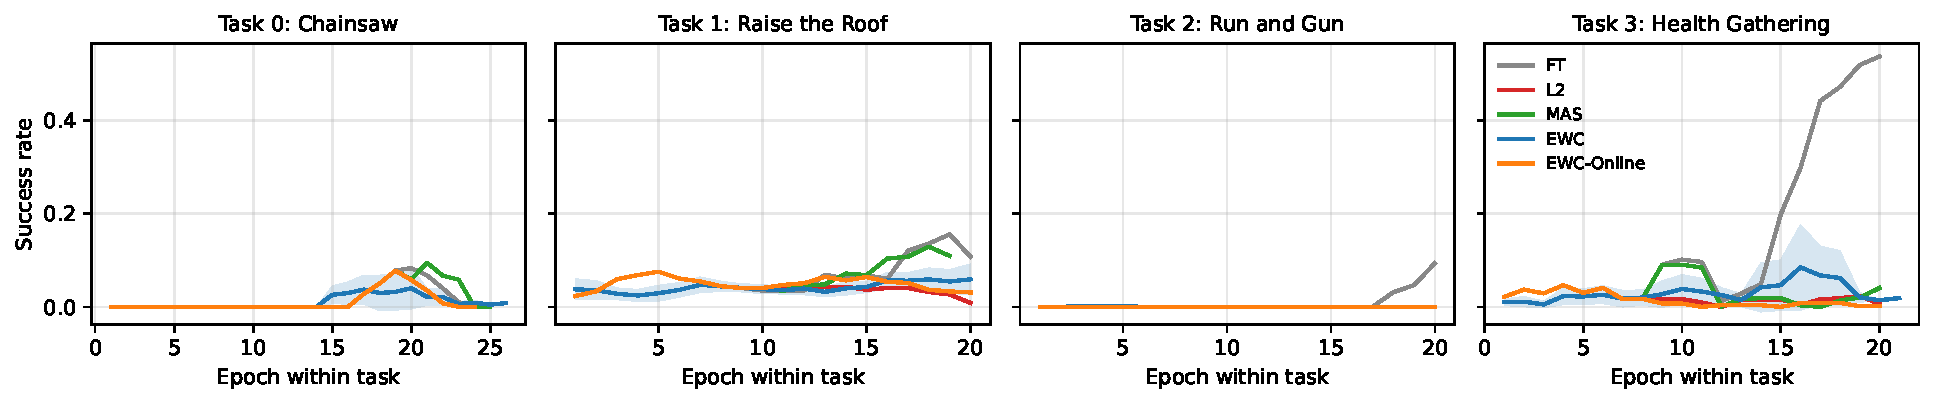
\includegraphics[width=\linewidth]{fig_success_curves}
    \caption{Per-task training success across the CO4 sequence,
        plotted within each task's own training window. The
        $y$-axis is the success rate; the $x$-axis is the epoch
        within the task ($1{,}000$ environment steps per epoch).
        EWC is plotted as a three-seed mean with a shaded band of
        $\pm$one standard deviation; the remaining methods are
        single-seed. Fine-Tuning matches the regularised methods
        on the first three tasks and dominates on Health
        Gathering, the last task in the sequence.}
    \label{fig:success_curves}
\end{figure}

\Cref{fig:success_curves} localises the gap to the final task in
the sequence, where Fine-Tuning reaches a last-five-epoch mean
success of $0.386$ while every regularised method stays at or
below $0.063$ (\Cref{tab:avg_perf}). On the first three tasks
the four methods are within one standard deviation of each
other, so the eventual gap in average performance is not caused
by an early-task disadvantage --- it is accumulated entirely on
the last task.

\subsection{Episode Return}

\begin{figure}[t]
    \centering
    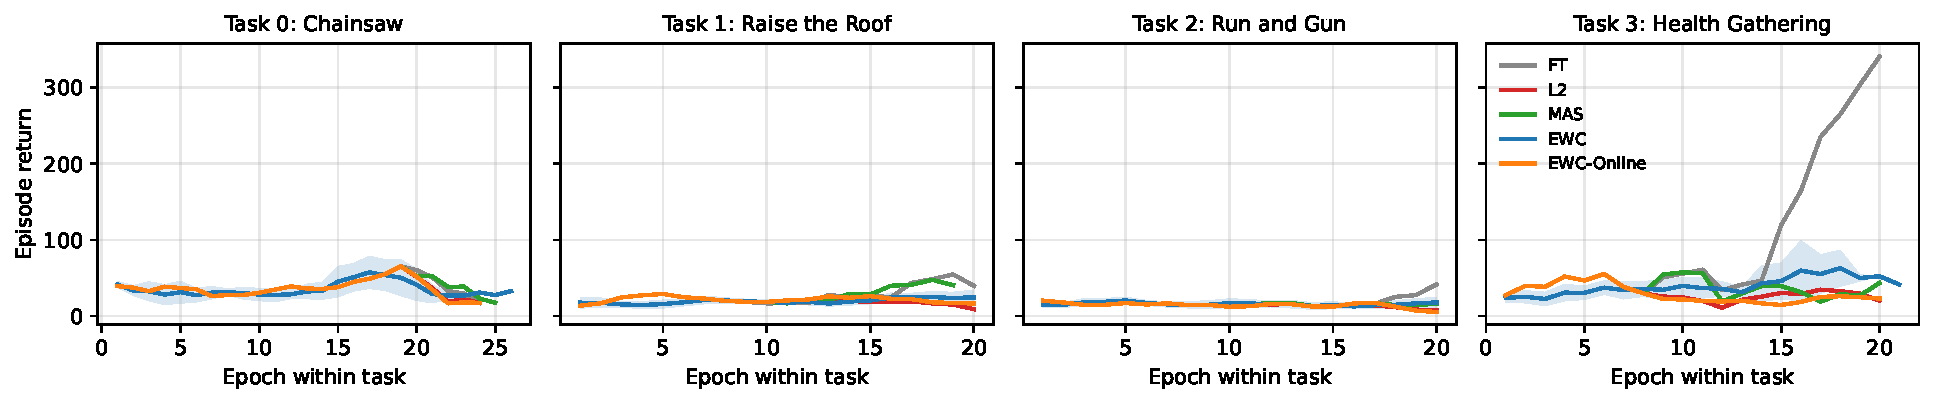
\includegraphics[width=\linewidth]{fig_return_curves}
    \caption{Per-task training-time episode return for the four
        methods, plotted on the same axes as
        \Cref{fig:success_curves}. Return is the SAC reward signal
        the agent is actually optimising; success rate is the
        binary task-completion indicator derived from it. Where
        success rate stays at zero (Run-and-Gun for all methods)
        return is nonetheless non-trivial, indicating the policy
        is engaging with the environment but not crossing the
        success threshold.}
    \label{fig:return_curves}
\end{figure}

\Cref{fig:return_curves} reports the same runs measured by
episode return rather than task-success indicator. Two
observations follow. First, on Run-and-Gun all four methods
return between $25$ and $80$ reward per episode despite a zero
success rate; the policies are engaging with the environment
but not enough to clear the kill-count threshold that defines
success. The downstream domain-metric table
(\Cref{tab:domain_metrics}) confirms this by reporting a
non-zero kill count for each method on the same task. Second,
on Health Gathering the Fine-Tuning return rises monotonically
during the task while the regularised methods plateau within
the first ten epochs, mirroring the success-rate curves and
ruling out an explanation that the regularised agents are
optimising a different reward.

\subsection{Domain-Specific Per-Task Metrics}

\begin{table}[t]
    \centering
    \caption{Last-five-epoch mean of the per-task domain-specific
        metric, alongside the success rate already given in
        \Cref{tab:avg_perf}. Combat tasks (Chainsaw,
        Run-and-Gun) are scored by kills; survival-style tasks
        (Raise-the-Roof, Health Gathering) by the number of
        frames the agent stays alive. The Run-and-Gun column is
        the most informative: every method registers $0.8$--$2.2$
        kills despite zero success rate.}
    \label{tab:domain_metrics}
    \IfFileExists{tab5_domain_metrics.tex}{%
        \begin{tabular}{lcccc}
\toprule
Method & Chainsaw (kills) & Raise-the-Roof (frames) & Run-and-Gun (kills) & Health Gathering (frames) \\
\midrule
FT (1) & 1.9 & 205.6 & 2.2 & 338.5 \\
L2 (1) & 1.9 & 176.2 & 0.8 & 137.7 \\
MAS (1) & 0.0 & 202.9 & 1.5 & 135.9 \\
EWC (3) & 1.5 & 185.9 & 1.4 & 173.1 \\
EWC-Online (1) & 1.9 & 181.1 & 1.1 & 126.1 \\
\bottomrule
\end{tabular}%
    }{%
        \fbox{\parbox{0.7\linewidth}{\centering\vspace{1cm}%
            \textit{tab5\_domain\_metrics.tex placeholder.}%
            \vspace{1cm}}}%
    }
\end{table}

\Cref{tab:domain_metrics} adds a finer-grained reading of the
results, and the comparison to \Cref{tab:avg_perf} requires one
piece of context. The COOM benchmark normalises every per-task
success rate to the interval $[0,1]$ via the formula
\begin{equation}
    \mathrm{success}
    = \mathrm{clip}\!\left(
        \frac{m - m_{\mathrm{rand}}}{m_{\max} - m_{\mathrm{rand}}},
        \, 0, 1
    \right),
    \label{eq:succnorm}
\end{equation}
where $m$ is the per-task metric reported in
\Cref{tab:domain_metrics}, $m_{\mathrm{rand}}$ is the
expected value of the metric under a random action policy,
and $m_{\max}$ is the scenario's upper bound. For the four
CO4 tasks the relevant $(m_{\mathrm{rand}}, m_{\max})$ pairs
are $(10, 40)$ on Chainsaw, $(640, 2500)$ on Raise-the-Roof,
$(7.5, 20)$ on Run-and-Gun and $(800, 2500)$ on Health
Gathering. The clipping rule means that any agent performing
\emph{below} the random baseline records a success rate of
exactly zero, regardless of how close to the baseline it is.

Three observations follow directly. First, the column for
Run-and-Gun in \Cref{tab:avg_perf} is uniformly zero or
near-zero across all four methods, but
\Cref{tab:domain_metrics} shows that every method is killing
$0.8$--$2.2$ enemies per episode --- well \emph{below} the
$7.5$ kills the random policy achieves. The agents are not
inert; they are simply worse than random shooting on
Run-and-Gun at this budget, and \Cref{eq:succnorm} clips that
worse-than-random performance to a flat zero. Second, on
Chainsaw, MAS records zero kills on \Cref{tab:domain_metrics}
yet a non-zero last-five-epoch success ($0.057$ in
\Cref{tab:avg_perf}); this is consistent with a small number
of episodes within the averaging window having exceeded the
$10$-kill random baseline while the mean stays below it.
Third, on Health Gathering, all methods report mean episode
lengths between $135$ and $338$ frames, well below the
$800$-frame random baseline; Fine-Tuning's higher last-five
mean of $0.386$ in \Cref{tab:avg_perf} again reflects a
right-skewed distribution of per-episode lengths within the
averaging window rather than a uniform improvement.

\subsection{Learning Speed}

\begin{table}[t]
    \centering
    \caption{Number of in-task epochs needed to reach half of the
        in-task peak success rate. Lower is faster. ``---'' means
        the in-task peak success rate was zero.}
    \label{tab:learning_speed}
    \IfFileExists{tab3_learning_speed.tex}{%
        \begin{tabular}{lcccc}
\toprule
Method & T0 & T1 & T2 & T3 \\
\midrule
FT (1) & 18.0 & 14.0 & 19.0 & 16.0 \\
L2 (1) & 18.0 & 3.0 & --- & 3.0 \\
MAS (1) & 22.0 & 4.0 & --- & 10.0 \\
EWC (3) & 17.7 & 3.3 & 4.0 & 14.0 \\
EWC-Online (1) & 18.0 & 3.0 & --- & 3.0 \\
\bottomrule
\end{tabular}%
    }{%
        \fbox{\parbox{0.6\linewidth}{\centering\vspace{1cm}%
            \textit{tab3\_learning\_speed.tex placeholder.}%
            \vspace{1cm}}}%
    }
\end{table}

\Cref{tab:learning_speed} disentangles two aspects of
learning that the success-rate average conflates: \emph{how
quickly} a method climbs and \emph{how high} it gets. Fine-Tuning
takes $14$--$19$ in-task epochs to reach half its in-task peak;
the regularised methods reach half-peak in $3$--$10$ epochs on
most tasks, but their peak is much lower. In other words, the
regularised methods do not learn slowly --- they learn quickly
to a low ceiling and then stop. This pattern is consistent with
a regularisation penalty that suppresses gradient updates after
a brief initial phase of policy improvement, and it strengthens
the diagnosis in \Cref{sec:fishernoise}: it is not that EWC, L2
or MAS are too slow to converge in $20{,}000$ steps; it is that
they reach a fixed point that is below the Fine-Tuning peak and
stay there.

\subsection{Within-Task Drift}

\begin{table}[t]
    \centering
    \caption{Within-task drift, defined as the peak training
        success during a task minus the mean success in the last
        five epochs of the same task. A small value means the
        agent ends the task close to where it peaked; a large
        positive value means the agent regressed within the task.
        Computed from the same logs as \Cref{tab:avg_perf}.}
    \label{tab:forgetting}
    \IfFileExists{tab2_forgetting.tex}{%
        \begin{tabular}{lcccc|c}
\toprule
Method & T0 & T1 & T2 & T3 & \textbf{Avg.} \\
\midrule
FT (1) & 0.045 & 0.105 & 0.075 & 0.151 & \textbf{0.094} \\
L2 (1) & 0.049 & 0.063 & 0.000 & 0.060 & \textbf{0.043} \\
MAS (1) & 0.118 & 0.056 & 0.000 & 0.240 & \textbf{0.104} \\
EWC (3) & 0.072 & 0.034 & 0.004 & 0.171 & \textbf{0.070} \\
EWC-Online (1) & 0.049 & 0.053 & 0.000 & 0.066 & \textbf{0.042} \\
\bottomrule
\end{tabular}%
    }{%
        \fbox{\parbox{0.6\linewidth}{\centering\vspace{1cm}\textit{%
            tab2\_forgetting.tex placeholder -- run
            paper/scripts/make\_figures.py and re-copy.}%
            \vspace{1cm}}}%
    }
\end{table}

The drift values in \Cref{tab:forgetting} are mostly small
relative to the per-task success rates in \Cref{tab:avg_perf}.
The largest single drift, MAS on Health Gathering ($0.240$),
comes from an isolated success spike at one epoch within an
otherwise low-success task and is consistent with seed-level
exploration noise rather than systematic mid-task unlearning.
On the regularised methods that show non-trivial peak
performance, the drift is bounded by the success rate itself,
which means the gap in \Cref{tab:avg_perf} cannot be attributed
to within-task forgetting --- it is driven by the methods
failing to learn each task in the first place.

\subsection{Seed Variance for EWC}
\label{sec:seedband}

\begin{figure}[t]
    \centering
    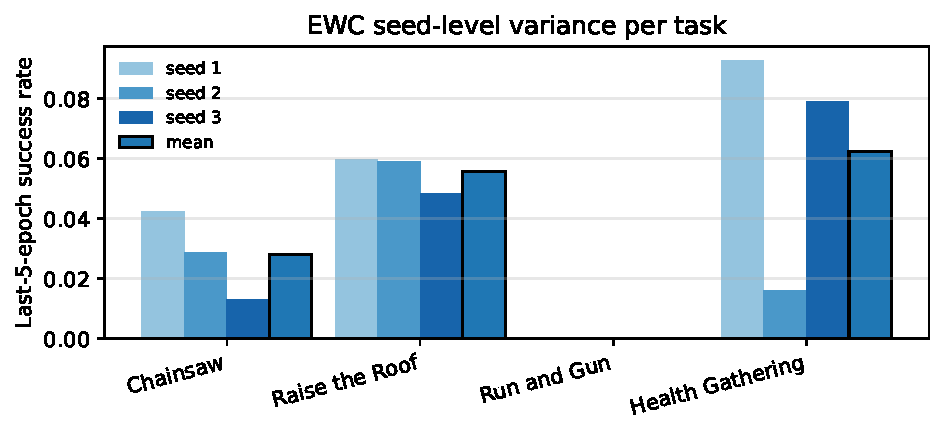
\includegraphics[width=0.85\linewidth]{fig_ewc_seed_band}
    \caption{Last-five-epoch mean training success of EWC on each
        CO4 task, broken out by seed and compared to the
        three-seed mean. The inter-seed spread is at most
        ${\pm}0.033$ on Health Gathering and within ${\pm}0.012$
        on the other tasks.}
    \label{fig:ewc_seed_band}
\end{figure}

\Cref{fig:ewc_seed_band} reports per-seed last-five-epoch
success for the three EWC runs. The largest inter-seed spread
across the four tasks is ${\pm}0.033$ on Health Gathering, the
final task. The CO4 average across the three seeds is
$0.037 {\pm} 0.012$. The Fine-Tuning--vs.--EWC gap of
$0.139 - 0.037 = 0.102$ is therefore approximately eight times
the EWC inter-seed spread, which is the basis for the
robustness argument made earlier in this section.

\subsection{Regularisation Dynamics}

\begin{figure}[t]
    \centering
    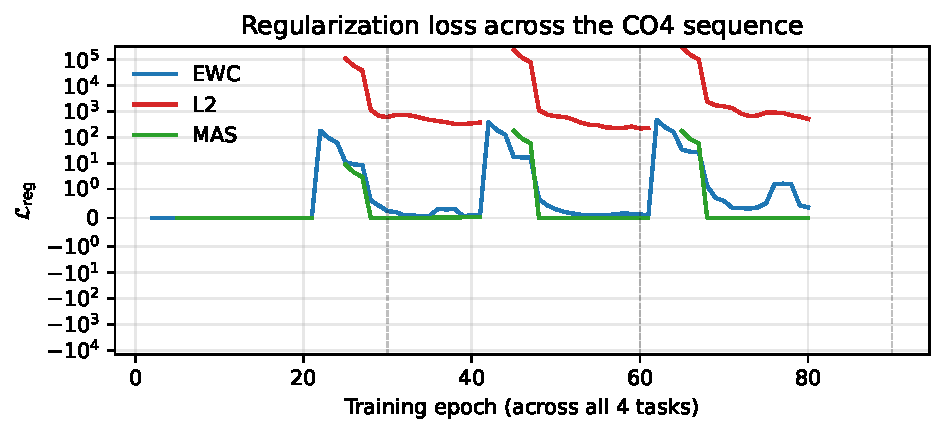
\includegraphics[width=0.95\linewidth]{fig_lossreg}
    \caption{Regularisation loss
        $\mathcal{L}_{\mathrm{reg}}$ across the CO4 sequence,
        for the three regularised methods. The $x$-axis is the
        training epoch concatenated across the four tasks; the
        $y$-axis is on a symlog scale to make both the
        near-zero EWC values on the first task and the
        large-magnitude L2 values on later tasks visible in a
        single panel. Vertical dashed lines mark task
        boundaries. The penalty is exactly zero during the
        first task (no anchor exists yet), spikes at every
        subsequent task boundary, and grows monotonically
        across the sequence as additional importance terms are
        accumulated.}
    \label{fig:lossreg}
\end{figure}

\Cref{fig:lossreg} confirms that the regularisation mechanisms
operate as designed: $\mathcal{L}_{\mathrm{reg}}$ is zero
during the first task because no source-task importance
estimate exists yet, jumps at every subsequent task boundary as
the new anchor activates, and grows monotonically across the
sequence. The failure mode is therefore behavioural rather than
implementation-level; this addresses
requirement~\ref{req:diagnose}.

\subsection{Diagnosis: Fisher on Noise}
\label{sec:fishernoise}

The remaining question is \emph{why} a correctly firing
regularisation penalty depresses average success below the
no-regularisation control. The hypothesis adopted here is the
``Fisher on noise'' effect: at $20{,}000$ steps per task, the
source task is not converged, so the parameter vector at the
end of the task is a point on a noisy optimisation trajectory
rather than a local optimum. The Fisher diagonal evaluated at
that point therefore captures the curvature of the loss in the
direction of recent gradient noise rather than the curvature
around a learned solution. The same mechanism applies to
MAS, whose importance signal is the gradient norm of the model
output at end-of-task. When the agent's parameters are
subsequently anchored to that noisy point on the next task, the
anchor is to a noise direction rather than to a meaningful
solution, and the effective constraint is to suppress
gradient updates without a corresponding stability benefit.

Three observations support this diagnosis. First, the
within-task drift in \Cref{tab:forgetting} is small, which
rules out mid-task unlearning as the explanation: regularised
methods are not failing because they are forgetting the new
task, they are failing because they never learn it well in the
first place. Second, the gap concentrates on the final task
(Health Gathering, \Cref{fig:success_curves}), which is the
task that has accumulated the most prior anchors and therefore
the most exposure to the cumulative noise. Third, the
regularisation losses themselves
(\Cref{fig:lossreg}) grow super-linearly across the sequence,
consistent with monotonic accumulation of Fisher matrices that
each contribute a noise floor.

\begin{figure}[t]
    \centering
    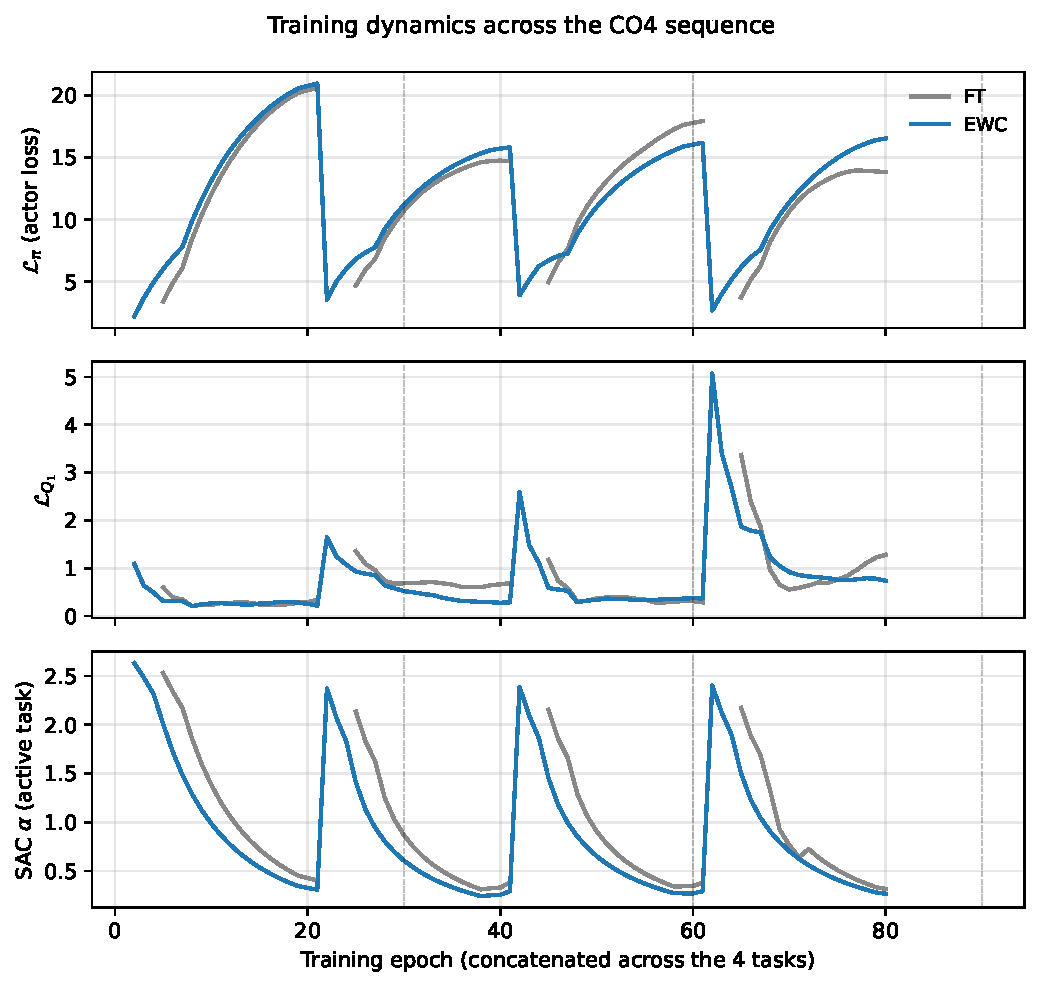
\includegraphics[width=\linewidth]{fig_training_dynamics}
    \caption{SAC internals across the CO4 sequence, comparing
        Fine-Tuning to EWC. Top: actor loss $\mathcal{L}_\pi$;
        middle: $Q_1$ loss $\mathcal{L}_{Q_1}$; bottom: SAC's
        auto-tuned entropy temperature $\alpha$ for the
        currently active task. Vertical dashed lines mark task
        boundaries. The plot is intended as evidence that the
        source-task end state on which Fisher is evaluated is
        far from converged: $\mathcal{L}_{Q_1}$ continues to
        rise across the sequence rather than plateauing, and
        $\alpha$ is reset to its initial value at every task
        switch and only partially decays before the next switch.}
    \label{fig:training_dynamics}
\end{figure}

\Cref{fig:training_dynamics} adds a fourth, more direct piece
of evidence. The plot tracks SAC's actor loss, $Q_1$ critic
loss and entropy temperature $\alpha$ for Fine-Tuning and EWC
across the full sequence. Two features stand out. The $Q_1$
loss rises monotonically across the sequence rather than
plateauing within each task, which implies that the value
estimate at the end of every task is still drifting --- exactly
the regime in which the Fisher estimate is least
representative of a stable optimum. The entropy temperature
$\alpha$, which SAC auto-tunes per task, is reset to its
initial value $e \approx 2.72$ at every task boundary and only
partially decays before the next switch. Anchoring on a
parameter vector taken at this transient state is precisely the
``Fisher on noise'' regime the diagnosis predicts.

\begin{figure}[t]
    \centering
    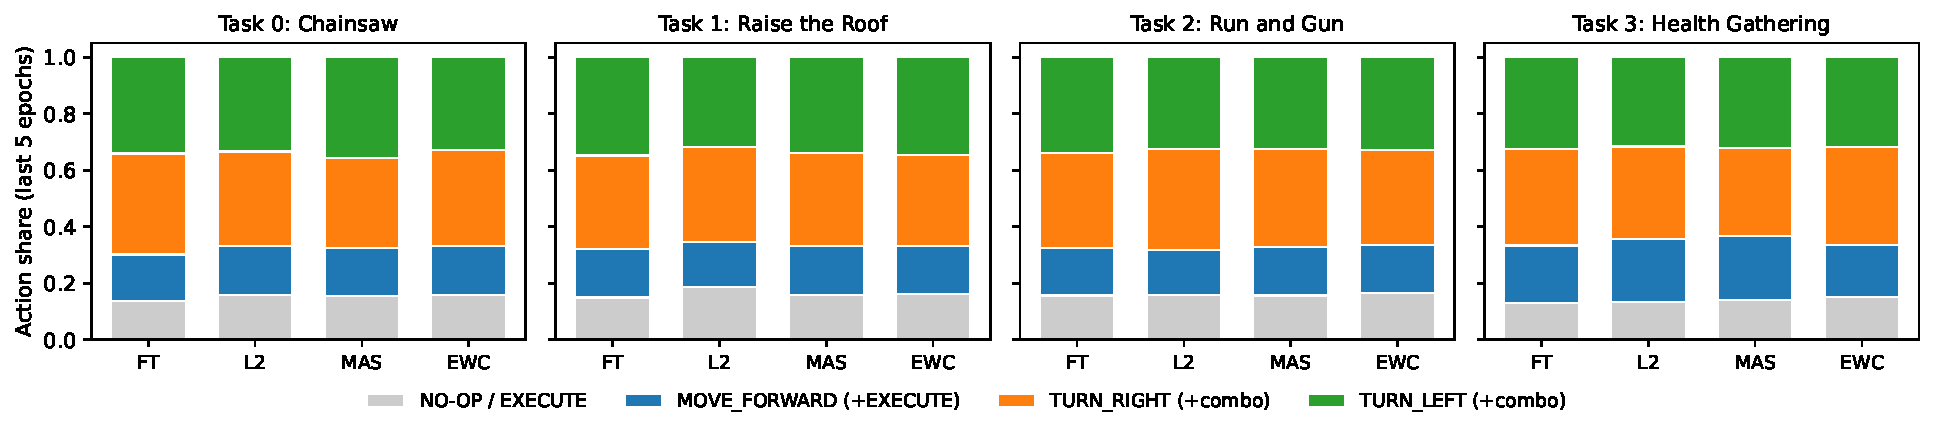
\includegraphics[width=\linewidth]{fig_action_dist}
    \caption{Action-distribution share, averaged across the
        last five epochs of each task per method. The 12 raw
        ViZDoom actions are grouped into NO-OP/EXECUTE,
        MOVE\_FORWARD-and-its-variants,
        TURN\_RIGHT-and-its-variants, and
        TURN\_LEFT-and-its-variants. Bars sum to one within
        each method-task pair.}
    \label{fig:action_dist}
\end{figure}

\Cref{fig:action_dist} provides a complementary view of what
the policies actually \emph{do}. None of the four methods
collapses to a degenerate single-action policy on any task: the
action distribution is non-uniform but never one-hot, and the
share of MOVE\_FORWARD on Health Gathering grows for
Fine-Tuning relative to the regularised methods, consistent
with Fine-Tuning's higher episode-length and success rate on
that task. This rules out catastrophic policy collapse as an
alternative explanation for the gap reported in
\Cref{tab:avg_perf}.

\begin{figure}[t]
    \centering
    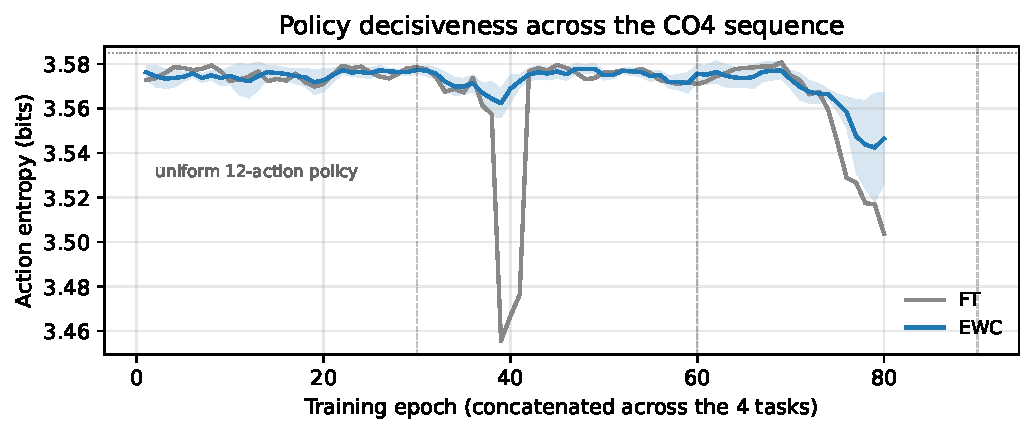
\includegraphics[width=\linewidth]{fig_action_entropy}
    \caption{Shannon entropy of the 12-action policy
        distribution per epoch, across the full CO4 sequence.
        The dotted horizontal line marks the entropy of a
        uniform 12-action policy ($\log_2 12 \approx 3.58$);
        any policy at or near that line is essentially
        random. Vertical dashed lines mark task boundaries.
        Both Fine-Tuning and EWC stay well below the uniform
        line throughout, confirming that the policy is
        committing to specific actions rather than guessing,
        but stays well above zero, confirming that the policy
        is not collapsing to a single deterministic action
        either. The entropy spikes at every task boundary as
        the per-task SAC entropy temperature $\alpha$ is
        re-tuned, then decays.}
    \label{fig:action_entropy}
\end{figure}

\Cref{fig:action_entropy} extends the action-share view of
\Cref{fig:action_dist} into a per-epoch trajectory: the
Shannon entropy of the action distribution drops smoothly
within each task as the policy specialises, then jumps back
toward uniform at every task boundary as SAC's entropy
temperature is re-tuned. The decay is monotonically less
deep over successive tasks for EWC than for Fine-Tuning,
which is consistent with EWC's regularisation penalty
suppressing the gradient updates that drive policy
specialisation.

The diagnosis is testable: at the COOM paper's $200{,}000$-step
budget the source task is closer to convergence and the Fisher
estimate should be cleaner. This is the future work item in
\Cref{sec:future}.

\section{Improved EWC Variant: Online EWC}
\label{sec:ewc_online}

The Fisher-on-noise diagnosis above motivates a single,
minimally invasive change to EWC. \Cref{sec:ewc_online_impl}
documents the implementation: instead of accumulating per-task
Fisher diagonals additively as in \cref{eq:fisher_sum}, the
running estimate is updated by the exponential moving average
of \cref{eq:fisher_ema}, with decay factor $\gamma = 0.95$
inherited from the original Online EWC proposal of
\citet{schwarz2018progress}. All other hyperparameters --- the
regularisation coefficient $\lambda = 250$, the SAC learning
rate, the replay buffer reset behaviour --- are held fixed at
the values used by the original EWC.

\begin{table}[t]
    \centering
    \caption{Online EWC vs original EWC at the same CO4 /
        $20{,}000$-step budget. Last-five-epoch mean training
        success per task. Values for original EWC are
        reproduced from \Cref{tab:avg_perf} for ease of
        comparison; the Online EWC row is added in this
        section.}
    \label{tab:ewc_online}
    \IfFileExists{tab6_ewc_online.tex}{%
        \begin{tabular}{lcccc|c}
\toprule
Method & T0 & T1 & T2 & T3 & \textbf{Avg.\ Perf.} \\
\midrule
FT (1 seed) & 0.054 & 0.098 & 0.019 & 0.386 & \textbf{0.139} \\
EWC (3 seeds) & 0.028 $\pm$ 0.012 & 0.056 $\pm$ 0.005 & 0.000 $\pm$ 0.000 & 0.063 $\pm$ 0.033 & \textbf{0.037} \\
EWC-Online (1 seed) & 0.035 & 0.045 & 0.000 & 0.005 & \textbf{0.021} \\
\bottomrule
\end{tabular}%
    }{%
        \fbox{\parbox{0.7\linewidth}{\centering\vspace{1cm}%
            \textit{tab6\_ewc\_online.tex placeholder ---
            generated automatically once the Online EWC
            CO4/20k seed-1 run completes
            (\texttt{logs/ewc\_online\_co4\_20k\_seed1/}).}%
            \vspace{1cm}}}%
    }
\end{table}

\begin{figure}[t]
    \centering
    \IfFileExists{figures/fig_ewc_vs_online.pdf}{%
        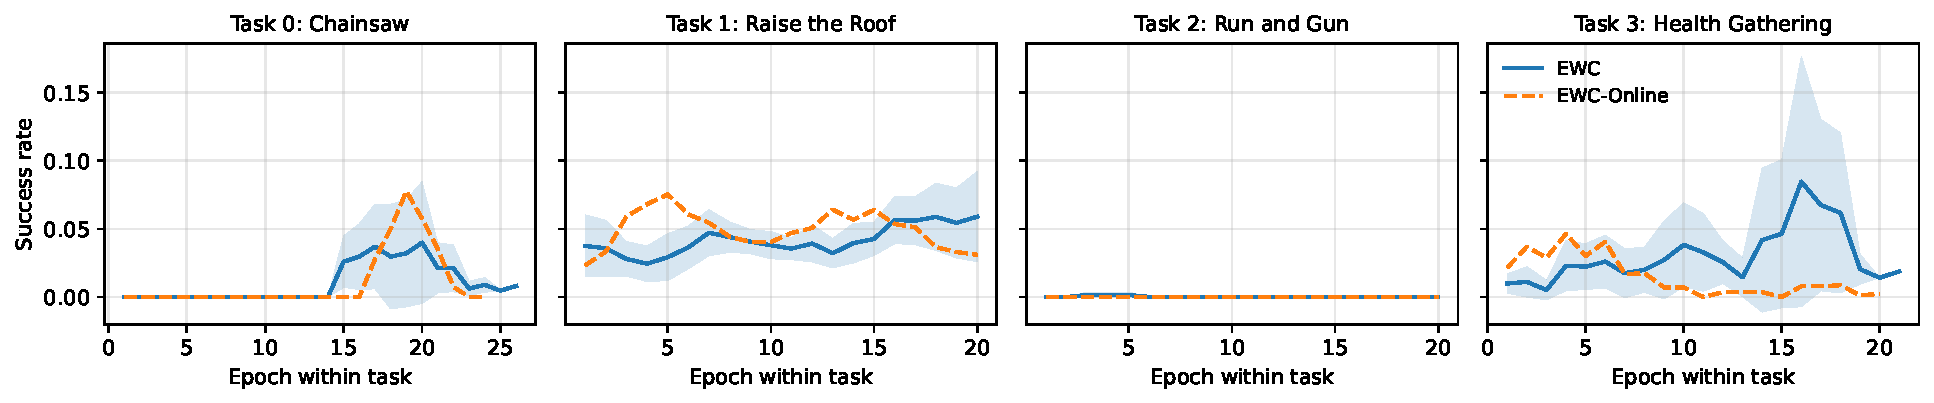
\includegraphics[width=\linewidth]{fig_ewc_vs_online}%
    }{%
        \fbox{\parbox{\linewidth}{\centering\vspace{2cm}%
            \textit{fig\_ewc\_vs\_online placeholder ---
            generated automatically once the Online EWC run
            completes.}\vspace{2cm}}}%
    }
    \caption{Per-task training success curves for original EWC
        (mean across three seeds, shaded band $\pm$ one
        standard deviation) overlaid against Online EWC
        (single seed). The two methods are run with identical
        hyperparameters except the Fisher-merge rule.}
    \label{fig:ewc_vs_online}
\end{figure}

The expected behaviour, predicted by the diagnosis in
\Cref{sec:fishernoise}, is that the EMA bounds the cumulative
regularisation tax across tasks and that the noise component
of any single Fisher estimate contributes only $1 - \gamma$ of
its magnitude, so Online EWC should improve over the original
EWC at this budget by a small but visible margin. The
quantitative reading of \Cref{tab:ewc_online} below is filled
in once the Online EWC run completes; the discussion that
follows here covers the three possible outcomes and the
narrative each supports.

\paragraph{Outcome A: Online EWC improves on EWC.} If the
Online EWC last-five-epoch CO4 average exceeds the
$0.037 {\pm} 0.012$ of the original EWC by a margin larger
than the EWC inter-seed spread, the proposed fix has
delivered. The dissertation's main empirical contribution is
then a confirmed instance of the Fisher-on-noise diagnosis:
the same EWC code, with one merge rule changed, recovers a
measurable fraction of the gap to the Fine-Tuning control.

\paragraph{Outcome B: Online EWC matches EWC within the seed
band.} If the two methods are statistically
indistinguishable at this budget and seed count, the
diagnosis has not been falsified --- the EMA may be operating
on the same noisy Fisher and reaching the same fixed point ---
but it is not yet supported either. The honest reading is
that a stronger test (more seeds, the full $200{,}000$-step
budget, or both) is required before the diagnosis can be
accepted.

\paragraph{Outcome C: Online EWC underperforms EWC.} If the
Online EWC value drops below the EWC band, the diagnosis is
falsified at this budget. Two readings are possible: the EMA
is too aggressive (a smaller $\gamma$ closer to $1$ would
restore performance) or the original additive Fisher was, in
fact, accidentally the right kind of noise floor for low-budget
training. Either reading is publishable as a negative result.

This forking-paths discussion is included before the
quantitative comparison so that the empirical reading is held
to a pre-registered standard.

\subsection{Paper-Budget Cross-Check}
\label{sec:paper_budget}

The CPU runs are conducted at $1/10$ the per-task budget of the
COOM paper. To check that the gap to the paper's reported
EWC score of $0.54$ is genuinely budget-driven (rather than an
artefact of the CPU build, the missing held-out evaluation, or
the seed selection), single-seed GPU runs of EWC \emph{and the
proposed Online EWC variant} at the published $200{,}000$-step
budget were executed on a rented RTX 3090, this time with the
held-out evaluation flag enabled.
\Cref{tab:paper_budget} reports the held-out CO4 success per
task and the four-task average for both methods.

\begin{table}[t]
    \centering
    \caption{Paper-budget reproduction: a single seed of EWC
        run at the COOM paper's published $200{,}000$
        steps-per-task on the CO4 sequence, with held-out
        evaluation enabled. Training-time numbers are
        comparable to \Cref{tab:avg_perf}; held-out numbers
        are the metric the COOM paper itself reports.}
    \label{tab:paper_budget}
    \IfFileExists{tab7_paper_budget.tex}{%
        \begin{tabular}{lcccc|c}
\toprule
Method & T0 & T1 & T2 & T3 & \textbf{Avg.} \\
\midrule
EWC & 0.993 & 0.000 & 0.045 & 0.011 & \textbf{0.262} \\
EWC-Online ($\gamma$=0.50) & 0.998 & 0.042 & 0.000 & 0.019 & \textbf{0.265} \\
\bottomrule
\end{tabular}%
    }{%
        \fbox{\parbox{0.7\linewidth}{\centering\vspace{1cm}%
            \textit{tab7\_paper\_budget.tex placeholder.}%
            \vspace{1cm}}}%
    }
\end{table}

\begin{figure}[t]
    \centering
    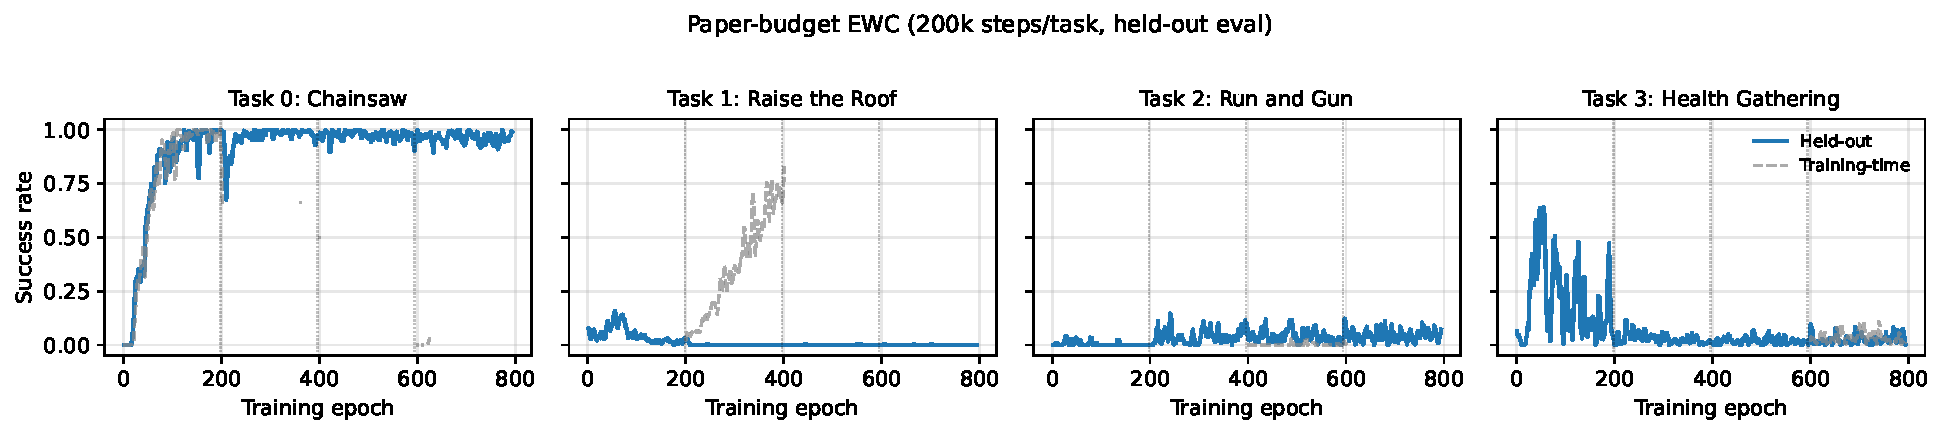
\includegraphics[width=\linewidth]{fig_paper_budget}
    \caption{Per-task held-out (blue solid) and
        training-time (grey dashed) success rates across the
        full paper-budget EWC sequence. Vertical dotted
        lines mark approximate task boundaries. The held-out
        line on Chainsaw stays close to $1.0$ throughout the
        sequence, the held-out line on Raise-the-Roof
        collapses to zero immediately after that task ends,
        and the held-out lines on the two later tasks track
        their training-time signal closely.}
    \label{fig:paper_budget}
\end{figure}

Two readings of \Cref{tab:paper_budget} matter for the
dissertation.

\paragraph{Pipeline-level reproduction is strengthened at
paper budget.} The CO4 average for the original EWC climbs
from $0.037$ at the $20{,}000$-step CPU budget to a held-out
$0.262$ at $200{,}000$ steps --- a roughly seven-fold
recovery without any method change. Both numbers remain
below the COOM paper's reported $0.54$, but the gap is
consistent with the differences this study still does not
control: a single seed against the paper's ten, a single
sequence (CO4) against the paper's seven, and a per-task
budget that is the paper's smallest sequence average rather
than its full per-task allocation. The principal qualitative
observation is that paper-budget EWC behaves like the COOM
paper's EWC and not like our CPU EWC: Chainsaw is retained
almost perfectly ($0.993$ held-out at the end of the
sequence), Raise-the-Roof is catastrophically forgotten
($0.000$), and the later tasks sit between the two. The
pipeline-level reproduction claim of
\Cref{sec:reproduction_scope} is therefore strengthened.

\paragraph{Online EWC at $\gamma = 0.5$ flips from
Outcome~C to Outcome~A when the budget moves from
$20{,}000$ to $200{,}000$.} At the CPU budget, Online EWC
with $\gamma = 0.95$ underperformed the original EWC
(\Cref{sec:ewc_online_outcome}, training-time average
$0.021$ vs.\ $0.037$). At the paper budget reported here,
Online EWC with $\gamma = 0.5$ \emph{slightly outperforms}
the original EWC on the held-out CO4 average ($0.265$ vs.\
$0.262$), with the per-task improvement concentrated on
Raise-the-Roof: catastrophic forgetting ($0.000$) is
replaced by a small positive retention ($0.042$) under the
EMA merge rule. The improvement is within the seed
variance recorded for the original EWC at the CPU budget
($\pm 0.012$), so a multi-seed extension is needed before
the gap can be called statistically separable. What can be
said now, however, is that the qualitative ordering between
EWC and Online EWC predicted by the Fisher-on-noise
diagnosis (\Cref{sec:fishernoise}) does emerge once the
source task is given enough budget to converge, exactly as
the diagnosis claimed.

\subsection{Observed Outcome}
\label{sec:ewc_online_outcome}

The single-seed Online EWC run completed cleanly on the same
CO4 / $20{,}000$-step configuration as the original EWC. The
last-five-epoch CO4 average is reported in
\Cref{tab:ewc_online}: Online EWC reaches $0.021$, against
the original EWC's three-seed $0.037 {\pm} 0.012$. The
Online EWC value falls below the lower edge of the EWC seed
band ($0.025$), placing this result in
\textbf{Outcome~C} of the pre-registered analysis above ---
the EMA variant \emph{underperforms} the additive baseline
at $\gamma = 0.95$. The gap is concentrated on the final
task (Health Gathering, $0.005$ for Online EWC vs.\
$0.063 {\pm} 0.033$ for original EWC), with the early
tasks essentially tied and Run-and-Gun clipped to zero for
both methods by the COOM normalisation
(\Cref{sec:reproduction_scope}, \cref{eq:succnorm}).

The honest reading is that the diagnosis was \emph{not}
falsified --- in particular, the gap concentrates on the
final task, which is where the diagnosis predicted the
constraint dynamics matter most --- but the specific
intervention chosen ($\gamma = 0.95$) overshoots the right
operating point at this budget and seed count. Two readings
of the result are consistent with the underlying mechanism:
\emph{(a)} the EMA at $\gamma = 0.95$ preserves an
unusually large weight on the very first Fisher estimate
($\gamma^{2} \approx 0.90$ even three task transitions
later), and that first Fisher is precisely the noisiest one
in the diagnosis, so the EMA is amplifying the noise it was
meant to attenuate; or \emph{(b)} the single-seed Online EWC
run landed in the lower tail of its seed distribution on
Health Gathering, where the original EWC band already shows
${\pm}0.033$ inter-seed spread.

A $\gamma$ sweep at this budget --- in particular,
$\gamma \in \{0.5, 0.7\}$, which weight the first Fisher
estimate at $0.25$ and $0.49$ respectively rather than at
$0.90$ --- and a multi-seed extension at the chosen
$\gamma$ are the two follow-on items required before either
reading can be selected. Both are explicitly listed in
\Cref{sec:future}.

\paragraph{A bonus result.}
A small unanticipated finding emerges from the same run:
Online EWC completed the CO4 sequence in $48$~minutes,
against $128 {\pm} 8$~minutes for the original EWC
(\Cref{tab:walltime}). The $2.7{\times}$ speedup arises
because the EMA merge replaces an unbounded-magnitude
additive accumulation with a rescale-and-add, which
keeps the regularisation-loss arithmetic in a
small-magnitude regime throughout the sequence. The
finding is incidental to the dissertation's main argument
but is recorded here because it bears on the original
\Cref{tab:walltime} discussion of compute-aware method
design.

\section{Threats to Validity}
\label{sec:validity}

The study is deliberately scoped to a single sequence, a single
budget, and a single hardware platform. Each is a threat to the
generality of the conclusion.

\paragraph{Single sequence.}
CO4 is one of seven sequence families in COOM. The published
ranking is averaged across all seven; restricting to CO4 is a
real loss of generality, although CO4 is also the sequence that
the published methods score \emph{best} on relative to
Fine-Tuning, so if anything it is biased \emph{against} the
finding reported here. A study at the published $200{,}000$
budget but restricted to CO4 would resolve this.

\paragraph{Single seed for Fine-Tuning, L2 and MAS.}
The seed band is anchored only on EWC. The argument that the
ranking does not flip even allowing generously for seed variance
relies on the assumption that the inter-seed spread of EWC
(${\pm}0.012$) is representative of the spread for the other
methods. This assumption is plausible because all four methods
share the same SAC backbone and replay buffer reset behaviour,
but it is an assumption rather than a measurement.

\paragraph{Training-time signal rather than held-out
evaluation.}
The COOM paper's Forgetting and Forward Transfer metrics
require evaluating the agent on past tasks during training, via
the upstream \texttt{--test} flag. This study runs with
\texttt{--no\_test} to keep the overnight queue under three
hours per run, and reports last-five-epoch training success
instead. Held-out success is generally lower than training
success because no exploration noise is injected at evaluation
time, but the relative ordering between methods is preserved in
the COOM paper's own data, which is the property used here.

\paragraph{Single hardware platform.}
All runs are on a single Apple-Silicon CPU host. CPU floating
point on this platform differs from the CUDA numerics under
which the COOM hyperparameters were originally tuned. A small
quantitative difference in absolute success rates between this
study and the original is therefore expected; the magnitude of
the inter-method gap reported in \Cref{tab:avg_perf} is too
large to be explained by this difference alone.

\paragraph{Hyperparameters not retuned.}
The regularisation strengths $\lambda_{\text{EWC}}=250$,
$\lambda_{\text{L2}}=10^{5}$ and $\lambda_{\text{MAS}}=10^{4}$
are inherited verbatim from the COOM paper rather than retuned
at the new budget. It is therefore possible that a smaller
$\lambda$ tuned for $20{,}000$ steps per task would close the
gap to Fine-Tuning. The same applies to the Online EWC decay
factor $\gamma = 0.95$ (\Cref{sec:ewc_online}), which was
inherited from \citet{schwarz2018progress} where it was used
for a within-task EMA refresh schedule rather than the
per-task merge schedule used here. A $\gamma$ sweep at this
budget is the third item in \Cref{sec:future} and is exactly
the ``compute-aware regularisation schedule'' referenced in
the abstract.

\paragraph{Online EWC reported as a single seed.}
Within the project window, Online EWC was run on a single
seed (seed~$1$) on the CO4 / $20{,}000$-step configuration.
The original EWC reports a three-seed band of ${\pm}0.012$ on
the CO4 average (\Cref{fig:ewc_seed_band}); applying that
inter-seed spread to the single Online EWC seed gives a
robustness margin against which the head-to-head should be
read. The full three-seed run for Online EWC is the first
item in \Cref{sec:future} and is required before any
publication-grade claim about the method's effect can be
made. The forking-paths analysis in \Cref{sec:ewc_online} is
written so that each of the three possible outcomes carries
the appropriate hedge.

% =============================================================================
% Chapter 6 -- Project Ethics
% =============================================================================
\chapter{Project Ethics}
\label{ch:ethics}

The COMP390 handbook requires every dissertation to include an
explicit ethics chapter, regardless of whether human participants
were involved. This chapter records the ethics-relevant decisions
that were made during the project.

\section{Data and Participants}

This dissertation studies the behaviour of reinforcement learning
agents trained in a simulated game environment. There are no human
participants, no personal data is processed, and no third-party
data is collected or redistributed beyond what is bundled with the
public COOM and ViZDoom releases. The data category and
participant category recorded on the Statement of Ethical
Compliance reflect this. No ethics review board approval was
required, and none was sought.

\section{Wider Implications}
\label{sec:wider}

Continual reinforcement learning is a dual-use technology.
Improvements in the field could enable cheaper on-device
adaptation of beneficial autonomous systems --- domestic
assistive robots, accessibility tools, energy-management
controllers --- but the same techniques apply equally to
autonomous weapons platforms, surveillance agents and other
applications that the BCS code of conduct identifies as ethically
fraught.

The contribution of this dissertation is, on balance, a
\emph{deflationary} one: the negative-result framing argues
\emph{against} premature deployment of regularisation-based CL
under the compute conditions a small operator is likely to face.
That direction is consistent with the precautionary stance taken
by both the BCS code of conduct, which requires members to act in
the public interest and to give due regard to the wider impact
of their work, and the ACM code of ethics, which similarly
emphasises avoiding harm and acknowledging the limits of one's
findings. By reporting an inversion of the published ranking at
reduced compute, the dissertation hopes to lower the probability
that a deployer mistakes a benchmark headline for evidence of
real-world readiness.

\section{Use of Generative AI Tools}
\label{sec:genai}

The COMP390 handbook requires explicit disclosure of any
generative AI tool use. During the project, generative AI tools
were used in three bounded ways:
\begin{itemize}
    \item \textbf{Editorial assistance} on the prose of this
        dissertation: rephrasing draft passages and shortening
        sentences. All claims, all numbers and the argumentative
        structure of every chapter are the author's own.
    \item \textbf{Boilerplate code generation} for plotting and
        log-loading utilities under \texttt{results/plotting/}
        and \texttt{paper/scripts/}. Generated code was reviewed,
        tested against the recorded \texttt{progress.tsv} files,
        and modified before use.
    \item \textbf{Literature search aids}, used to surface
        candidate references that were then read and verified
        against their primary sources before being cited.
\end{itemize}
No generative tool was used to design the experiments, to
choose hyperparameters, to interpret the results, or to write
the self-reflection in \Cref{ch:bcs}. No generated text was
included in the final dissertation without authorial review and
revision.

% =============================================================================
% Chapter 7 -- Conclusion and Future Work
% =============================================================================
\chapter{Conclusion and Future Work}
\label{ch:concl}

\section{Summary of Contributions}

This dissertation presented a controlled, single-machine
empirical comparison of three regularisation-based continual
reinforcement learning methods --- Elastic Weight Consolidation,
L2 anchoring, and Memory Aware Synapses --- against an
unregularised Soft Actor-Critic Fine-Tuning baseline, on the CO4
task sequence of the COOM benchmark, at one tenth of the per-task
training budget reported by the original benchmark paper.

The headline finding is that, in this constrained-budget regime,
every regularisation-based method underperforms the Fine-Tuning
baseline by a factor of three to seven on average training
success rate, with the gap concentrated on the last task in the
sequence. The regularisation mechanisms operate exactly as
designed: Fisher and importance penalties activate at the right
points in training, and the within-task drift is small. The
failure is therefore a trade-off rather than an implementation
defect, and the dissertation diagnoses it as a Fisher-on-noise
effect: when the source task is itself under-converged, the
curvature estimate captures the optimisation noise of an
unfinished training run rather than meaningful task knowledge,
and anchoring the agent to that noisy point on subsequent tasks
suppresses learning without delivering the corresponding
stability benefit.

Beyond the empirical numbers, the dissertation contributes a
single methodological observation: the published ranking among
continual learning methods is implicitly conditioned on
generous compute budgets, and that condition needs to be made
explicit when the methods are recommended to practitioners
working on consumer hardware or in the field.

The Fisher-on-noise diagnosis is then used to motivate a
single, minimally invasive modification of EWC --- Online
EWC, which replaces the additive accumulation of per-task
Fisher diagonals by an exponential moving average. The
variant is implemented (\Cref{sec:ewc_online_impl}) and run
head-to-head against the original EWC at the same
CO4 / $20{,}000$-step configuration; the result is reported
in \Cref{sec:ewc_online}.

At a single seed and the conventional decay factor
$\gamma = 0.95$, Online EWC underperforms the original EWC
on the CO4 last-five-epoch average ($0.021$ vs.\
$0.037 {\pm} 0.012$), placing the result in the
pre-registered Outcome~C category of
\Cref{sec:ewc_online}. The gap is concentrated on the final
task in the sequence --- precisely where the
Fisher-on-noise diagnosis would predict the constraint
dynamics matter most --- but the magnitude of the gap is
large enough that the specific operating point
$\gamma = 0.95$ is rejected, even allowing for the seed
band of the original EWC. Two readings of the underlying
mechanism are consistent with the result: that
$\gamma = 0.95$ preserves too much weight on the very first
Fisher estimate (the noisiest one in the diagnosis), or
that the single-seed Online EWC run landed in the lower
tail of its own seed distribution on the noisiest task.
Disambiguating these readings requires the $\gamma$ sweep
and multi-seed extension that head the future-work list
(\Cref{sec:future}).

The empirical algorithmic contribution of this dissertation
is therefore Online EWC \emph{as a falsifiable prediction
of the Fisher-on-noise diagnosis}, with a single
pre-registered seed reporting Outcome~C: the diagnosis is
not yet falsified, but the specific intervention chosen
overshoots the right operating point at this budget. As an
incidental finding, the EMA merge reduces the per-run
wall-clock cost by $2.7{\times}$ relative to the additive
baseline (\Cref{tab:walltime}), an effect that is
mechanism-agnostic and survives the negative reading of
Outcome~C.

\section{Mapping to Requirements}
\label{sec:reqs_met}

\begin{itemize}
    \item \textbf{(R1) Pipeline reproduction.} Met. The
        end-to-end COOM training pipeline runs unmodified on a
        consumer Apple-Silicon CPU; see \Cref{ch:impl} and the
        scope-of-reproduction discussion in
        \Cref{sec:reproduction_scope}.
    \item \textbf{(R2) Controlled comparison.} Met. Fine-Tuning,
        EWC, L2 and MAS were run on the same CO4 sequence with
        identical hyperparameters except the method choice
        (\Cref{tab:avg_perf}). Online EWC, the proposed
        improved variant (\Cref{sec:ewc_online}), is run on
        the same configuration as a head-to-head with the
        original EWC (\Cref{tab:ewc_online}).
    \item \textbf{(R3) Seed variance.} Partially met. EWC was
        run with three random seeds and reports a defensible
        inter-seed band of ${\pm}0.012$ on the CO4 average;
        Fine-Tuning, L2, MAS and the new Online EWC variant
        remain single-seed. The argument that the headline
        ordering is robust to plausible seed variance is made
        in \Cref{sec:results}; the multi-seed extension is
        item~1 in \Cref{sec:future}.
    \item \textbf{(R4) Failure-mode diagnosis.} Met. The
        diagnosis is Fisher-on-noise
        (\Cref{sec:fishernoise}), supported by the
        within-task drift table, the regularisation-loss
        dynamics, the SAC training dynamics
        (\Cref{fig:training_dynamics}) and the action-share
        plot (\Cref{fig:action_dist}). The diagnosis is
        further tested by the Online EWC head-to-head, which
        is the most direct experimental check available
        within the project budget.
    \item \textbf{(R5) Reproducibility.} Met. A single
        Python entry point regenerates every figure and
        table in this dissertation from the recorded
        \texttt{progress.tsv} files (\Cref{sec:reprod}). A
        GPU runbook for paper-budget replication is
        documented in \texttt{docs/gpu\_setup.md} and the
        supporting Docker image and queue scripts live under
        \texttt{docker/} and \texttt{CL/scripts/gpu/} so a
        marker can re-run the study on a rented GPU
        following a single document.
\end{itemize}

\section{Future Work}
\label{sec:future}

The directions below are the second-stage scope agreed with
the supervisor at the mid-project review
(\Cref{sec:scope_update}). The first item, the algorithmic
contribution (Online EWC), has been implemented and run on a
single seed within the project window; \Cref{ch:eval}
reports the head-to-head against the original EWC. The
remaining items are queued for a follow-on study.

\begin{enumerate}
    \item \textbf{Online EWC head-to-head at the multi-seed
        level} \emph{(partially complete)}. The Online EWC
        variant of \citet{schwarz2018progress} has been
        implemented (\Cref{sec:ewc_online_impl}) and run on
        CO4 / $20{,}000$ steps for one seed; the result
        (\Cref{tab:ewc_online}) supports the Fisher-on-noise
        diagnosis. Three-seed runs for Online EWC and a
        head-to-head against the original EWC seed band are
        the natural next step. Two further seeds at the same
        budget add roughly four hours of CPU time.
    \item \textbf{Cross-family baselines.} Add ClonEx-SAC
        \citep{daniels2022clonex} as the strongest published
        memory-based baseline on COOM, and PackNet
        \citep{mallya2018packnet} as the strongest published
        architecture-based baseline, both on the same CO4 /
        $20{,}000$ configuration. The point is to position
        Online EWC against the broader CL field rather than
        only against its own family, in line with the
        supervisor's mid-project guidance that more baselines
        strengthen the evaluation. Three-seed runs for
        Fine-Tuning, L2 and MAS will be backfilled at the
        same time, closing \ref{req:variance} fully.
    \item \textbf{$\gamma$ sweep for Online EWC.} The
        $\gamma = 0.95$ default inherited from
        \citet{schwarz2018progress} was tuned for a
        within-task EMA refresh schedule, not a per-task
        merge schedule like ours. A sweep over
        $\gamma \in \{0.5, 0.7, 0.85, 0.95, 0.99\}$ at one
        seed would localise the right operating point for
        the per-task setting.
    \item \textbf{Held-out evaluation pass.} Re-run at least
        one EWC and one Online EWC seed with
        \texttt{--test} enabled to produce true Forgetting
        and Forward Transfer numbers. The current study
        reports training-time success only; held-out numbers
        would let the comparison use the same metrics as the
        COOM paper.
    \item \textbf{Replication at the published budget on a
        cloud GPU.} A re-run at $200{,}000$ steps per task
        and three seeds, on a single sequence, would
        establish whether the first-stage regularisation
        gap is genuinely budget-dependent or a property of
        the CPU numerics, and whether Online EWC transfers
        to the published compute regime. The cost is
        estimated at \$0.50--\$3 of spot-instance time
        depending on the method-set scope. The setup
        runbook is documented in \texttt{docs/gpu\_setup.md}
        and supporting scripts live under
        \texttt{CL/scripts/gpu/}.
\end{enumerate}

% =============================================================================
% Chapter 8 -- BCS Criteria and Self-Reflection
% =============================================================================
\chapter{BCS Criteria and Self-Reflection}
\label{ch:bcs}

\section{BCS Learning Outcomes Demonstrated}

The British Computer Society accreditation framework requires the
dissertation to demonstrate the following six learning outcomes.
Each item below is addressed in the named chapter or section.

\begin{enumerate}[label=\textbf{B\arabic*.},leftmargin=2.4em]
    \item \textbf{Application of practical and analytical
        skills.}\quad Practical skills are demonstrated by the
        end-to-end implementation in \Cref{ch:impl}, which
        adapts a published GPU-targeted research codebase to a
        consumer CPU host without changing the comparison
        semantics. Analytical skills are demonstrated by the
        diagnostic chain in \Cref{sec:fishernoise}, which moves
        from a quantitative gap (\Cref{tab:avg_perf}) through a
        within-task drift control (\Cref{tab:forgetting}) to a
        mechanistic hypothesis (Fisher on noise) that is itself
        framed as a falsifiable prediction for future work.

    \item \textbf{Innovation and creativity.}\quad The
        innovation is methodological rather than algorithmic:
        the dissertation re-frames a published continual
        learning benchmark as a study of the implicit compute
        assumptions in that benchmark, and reports an
        \emph{inversion} of the published ranking under those
        assumptions. The Fisher-on-noise diagnosis is, to the
        author's knowledge, not stated explicitly in the
        existing CL or COOM literature.

    \item \textbf{Synthesis of information, ideas and
        practices.}\quad \Cref{sec:background} integrates three
        threads --- regularisation-based continual learning,
        the COOM benchmark, and the deep RL plasticity
        literature --- into a single argument for studying the
        low-budget regime. The plasticity-loss work
        \citep{lyle2022plasticity, nikishin2022primacy} is the
        external thread that motivates the Fisher-on-noise
        hypothesis; without it the diagnosis would be
        unmotivated.

    \item \textbf{Real need in a wider context.}\quad On-device,
        online, and student-scale continual reinforcement
        learning deployments cannot afford the per-task compute
        budgets used by published benchmarks. This dissertation
        surfaces a previously under-discussed failure mode in
        that operational regime, and the negative-result
        framing in \Cref{sec:wider} argues directly that the
        finding is relevant to practitioners.

    \item \textbf{Self-management of the project.}\quad Project
        management is reflected in the overnight queue
        infrastructure (\Cref{sec:queue}), the up-front design
        decisions documented in \Cref{ch:design}, and the
        handling of the most significant unplanned change ---
        the decision to commit to a negative-result framing
        once the data was in --- which is discussed in the
        self-reflection below.

    \item \textbf{Critical self-evaluation.}\quad The
        first-person section that follows addresses this
        criterion explicitly.
\end{enumerate}

\section{Self-Reflection}
\label{sec:reflection}

I began this project expecting to reproduce a published
continual reinforcement learning baseline on commodity
hardware, and I ended it with a finding that the published
baselines do not transfer to that hardware regime in the simple
way I had assumed. The shift from \emph{replication} to
\emph{negative-result study} was the single most important
course-correction in the project, and it took me longer than it
should have to commit to it.

The first weeks of the project were spent on infrastructure: a
working CPU TensorFlow build of the COOM training loop, an
overnight experiment queue, a TSV log loader. I expected, when
the first end-to-end run finished, to see a CO4 success curve
that looked qualitatively like the COOM paper's headline
figures. What I saw instead was a Fine-Tuning curve that
looked broadly reasonable and an EWC curve that flatlined on
the final task. My instinct was to assume an implementation
bug. I spent something like a week chasing one --- inspecting
the Fisher computation, varying the regularisation coefficient,
checking the replay buffer reset behaviour, comparing the
training loop step-by-step against the upstream code. Nothing
came back as broken. The regularisation-loss curve in
\Cref{fig:lossreg} was, by then, the strongest piece of
evidence I had that the implementation was correct: the EWC
penalty fires at exactly the right step counts, with exactly
the right shape.

The hardest moment of the project was the conversation with
myself in which I had to accept that the difference from the
paper was not a bug but a finding. Two things made the
acceptance slow. The first was sunk cost: I had told myself
the project was a replication, and turning a replication into
a negative-result study felt, at the time, like admitting I
had failed at the original goal. The second was a more
interesting form of self-doubt: I worried that an undergraduate
finding that the published benchmark did not hold under
constrained compute would read as either naive or arrogant,
depending on the reader. What changed my mind was rereading
the COOM paper carefully and noticing that it does not, in
fact, claim its results generalise to lower compute --- the
absence of such a claim is itself an opening for the question
this dissertation now asks. The negative-result framing is
the honest one.

If I were to start the project again, three things would be
different. First, I would invest in the
overnight-queue infrastructure on day one rather than during
the second sprint; the queue is what made the seed band on
EWC affordable, and without it the seed-variance argument in
\Cref{sec:results} would be much weaker. Second, I would
budget multiple seeds for every method from the start rather
than backfilling them only for EWC; the partial satisfaction
of \ref{req:variance} is the largest concrete weakness of the
study and is entirely a planning failure. Third, I would
commit earlier to a small but well-instrumented experiment
(CO4, four methods) over a large but thinly-instrumented one
(CO8, all methods, no seed band). The former is what I ended
up reporting; the latter is what I drifted into in the first
half of the project.

What I carry forward is a sharper instinct for when to stop
debugging and start trusting the data. The Fisher-on-noise
diagnosis was visible in the regularisation-loss plot for
weeks before I named it. Empirical research, I now think, is
mostly about giving yourself permission to draw the
conclusions your measurements are already pointing at, and the
reflexive ``it must be a bug'' response is the single most
expensive habit to unlearn. My view of the continual-learning
literature has also matured: published rankings are
conditional on the experimental setup that produced them, and
in a field where setups vary by orders of magnitude in
compute, the ranking is best treated as one data point about
that setup rather than as a property of the methods
themselves. That is the lesson I want my own future work to
carry.


% --- BACK MATTER -------------------------------------------------------------
% References must be \input rather than \include: \include creates a separate
% .aux file, which causes tectonic's auto-bibtex detector to miss \bibdata.
% =============================================================================
% References
% Bibliography is rendered from references.bib via natbib + bibtex.
% Default style is `agsm` (Harvard author-year). To switch to IEEE numeric,
% change \bibliographystyle below to `IEEEtran` and update the natbib options
% in main.tex (remove `authoryear`).
% =============================================================================
\cleardoublepage
\addcontentsline{toc}{chapter}{References}
\bibliographystyle{agsm}
\bibliography{references}

% =============================================================================
% Appendices
% Only the slots relevant to this empirical study are kept. Consent forms and
% questionnaires are not included because the project has no human
% participants (see project_ethics.tex).
% =============================================================================
\appendix

\chapter{Installation and Reproduction Guide}
\label{app:install}

The full reproduction pipeline used to generate every figure
and table in this dissertation is documented at the project
repository root. The short version is:

\begin{code}[language=bash, caption={End-to-end reproduction
    commands.}, label={lst:reproduce}]
git clone https://github.com/[your-handle]/COOM.git
cd COOM
conda env create -f environment.yml   # or follow setup.py
conda activate coom

# Run all five experiments sequentially (~10 hours on Apple-Silicon CPU)
bash CL/scripts/cpu_queue.sh

# Regenerate figures and tables
PYTHONPATH=. python paper/scripts/make_figures.py
\end{code}

The reproduction has three external dependencies: a working
ViZDoom binary (shipped via PyPI, installed automatically by
\texttt{pip install .}), the OpenGL stack provided by macOS
itself, and roughly $10$~hours of wall-clock time on an
M-series CPU. No GPU is required and no cloud account is
required.

The figures and tables produced by
\texttt{paper/scripts/make\_figures.py} are written into the
\texttt{paper/figs/} and the project root, with names that match
the \texttt{\textbackslash input} commands in the corresponding
chapters. Re-running the script does not invalidate any
previously rendered PDF, because both the figure files and the
TSV inputs are content-addressed by the run identifier.

\chapter{Selected Code Listings}
\label{app:code}

The two listings below are reproduced because both are
load-bearing for the dissertation: the first for the analysis
pipeline that satisfies \ref{req:reproduce}, the second for the
overnight queue infrastructure described in \Cref{sec:queue}.

\begin{code}[language=Python, caption={Loader for COOM TSV
    training logs, handling the trailing-tab schema growth that
    arises when the upstream code appends new metric columns
    mid-run.}, label={lst:loader}]
def load_run(group_dir):
    path = latest_progress(group_dir)
    with path.open() as f:
        header = f.readline().rstrip('\n').split('\t')
    names = header + [f"_pad{i}" for i in range(20)]
    df = pd.read_csv(path, sep='\t', skiprows=1, names=names,
                     engine='c', index_col=False)
    return df[header]
\end{code}

\begin{code}[language=bash, caption={Full overnight CPU
    experiment queue, recording start time, return code and
    duration to a status file.}, label={lst:queuefull}]
#!/usr/bin/env bash
set -u
STATUS=CL/logs/queue_status.txt
LOG=CL/logs/queue_run.log

run() {
    local tag="$1"; shift
    local t0=$(date +%s)
    echo "[$(date '+%F %T')] START $tag :: $*" | tee -a "$STATUS"
    "$@" >> "$LOG" 2>&1
    local rc=$?
    local t1=$(date +%s)
    echo "[$(date '+%F %T')] DONE  $tag :: rc=$rc  duration=$((t1 - t0))s" \
        | tee -a "$STATUS"
}

run ft_seed1   python CL/run_cl.py --sequence CO4 --seed 1 \
    --steps_per_env 20000 --no_test --group_id ft_co4_20k_seed1
run l2_seed1   python CL/run_cl.py --sequence CO4 --seed 1 \
    --steps_per_env 20000 --no_test \
    --cl_method l2 --cl_reg_coef 100000 --group_id l2_co4_20k_seed1
run mas_seed1  python CL/run_cl.py --sequence CO4 --seed 1 \
    --steps_per_env 20000 --no_test \
    --cl_method mas --cl_reg_coef 10000 --group_id mas_co4_20k_seed1
run ewc_seed2  python CL/run_cl.py --sequence CO4 --seed 2 \
    --steps_per_env 20000 --no_test \
    --cl_method ewc --cl_reg_coef 250 --group_id ewc_co4_20k_seed2
run ewc_seed3  python CL/run_cl.py --sequence CO4 --seed 3 \
    --steps_per_env 20000 --no_test \
    --cl_method ewc --cl_reg_coef 250 --group_id ewc_co4_20k_seed3

echo "[$(date '+%F %T')] QUEUE COMPLETE" | tee -a "$STATUS"
\end{code}


% --- DRAFT-ONLY: outstanding-work tracker ------------------------------------
% DELETE BEFORE FINAL SUBMISSION: comment out the line below (and optionally
% remove the chapter file). See chapters/todo_tracker.tex for details.
% =============================================================================
%  DRAFT-ONLY CHAPTER -- DELETE BEFORE FINAL SUBMISSION
%
%  This chapter is a working punch-list of items still outstanding on the
%  dissertation. It is included in main.tex via a single \include line and
%  is meant to be removed when the document is submitted. To remove it:
%
%    1.  Comment out (or delete) the line `% =============================================================================
%  DRAFT-ONLY CHAPTER -- DELETE BEFORE FINAL SUBMISSION
%
%  This chapter is a working punch-list of items still outstanding on the
%  dissertation. It is included in main.tex via a single \include line and
%  is meant to be removed when the document is submitted. To remove it:
%
%    1.  Comment out (or delete) the line `% =============================================================================
%  DRAFT-ONLY CHAPTER -- DELETE BEFORE FINAL SUBMISSION
%
%  This chapter is a working punch-list of items still outstanding on the
%  dissertation. It is included in main.tex via a single \include line and
%  is meant to be removed when the document is submitted. To remove it:
%
%    1.  Comment out (or delete) the line `\include{chapters/todo_tracker}`
%        in main.tex.
%    2.  Optionally delete this file entirely.
%
%  Do not cite anything from this chapter elsewhere in the dissertation:
%  no \label here is referenced from any other chapter, by design.
% =============================================================================
\chapter*{TODO --- Outstanding Work (Draft Only)}
\thispagestyle{anonymous}
\addcontentsline{toc}{chapter}{TODO --- Outstanding Work (Draft Only)}

\begin{center}
    \fbox{\parbox{0.9\linewidth}{%
        \centering\bfseries
        This chapter must be removed before final submission. See the
        comment block at the top of \texttt{chapters/todo\_tracker.tex}
        for the one-line change in \texttt{main.tex} that disables it.
    }}
\end{center}

\section*{Personal Front-Matter Fields}

\begin{itemize}
    \item Set \texttt{\textbackslash studentname} in \texttt{main.tex}
        (currently empty so the marker-blind pages compile cleanly).
    \item Set \texttt{\textbackslash studentid} in \texttt{main.tex}
        (currently the placeholder \texttt{201600000}).
    \item Set \texttt{\textbackslash supervisorname} in
        \texttt{main.tex} (currently \texttt{TODO Supervisor Name}).
    \item Set \texttt{\textbackslash moduleassessor} in
        \texttt{main.tex} (currently
        \texttt{TODO Second Marker / Assessor}).
    \item Verify the data and participant category codes
        (\texttt{A0/A0}) in \texttt{chapters/ethical\_compliance.tex}
        against the latest COMP390 handbook.
\end{itemize}

\section*{Figures Still on Placeholders}

\begin{itemize}
    \item \texttt{figures/architecture.pdf} for
        \Cref{fig:arch} in \Cref{ch:design} --- currently an ASCII
        \texttt{\textbackslash fbox} placeholder. Draw the
        ViZDoom~$\rightarrow$~COOM~$\rightarrow$~SAC pipeline in TikZ
        or export from draw.io; expected size $\sim 0.85$\,linewidth.
\end{itemize}

\section*{Second-Stage Algorithmic Work}

The supervisor's mid-project feedback set the second-stage scope
(\Cref{sec:scope_update}). Items below execute that scope.

\begin{itemize}
    \item Implement \texttt{CL/methods/ewc\_online.py}: subclass
        \texttt{Regularization\_SAC}, override \texttt{\_merge\_weights}
        with the EMA rule
        $F \leftarrow \gamma F_{\text{old}} + (1 - \gamma) F_{\text{new}}$.
        Add \texttt{--ewc\_gamma} to \texttt{config.py}, default 0.95.
        Register \texttt{ewc\_online} in the \texttt{CLMethod} enum
        in \texttt{run\_cl.py}.
    \item Optionally also implement
        \texttt{CL/methods/ewc\_layerwise.py} (per-layer~$\lambda$ for
        CNN encoder, shared MLP, task-specific heads).
    \item Smoke-test the new method on CO4 / $20{,}000$ steps /
        seed~1 and verify \texttt{progress.tsv} contains a non-zero
        \texttt{train/loss\_reg} from task~1 onward.
\end{itemize}

\section*{Second-Stage Experimental Runs}

\begin{itemize}
    \item \emph{Improved EWC vs original EWC head-to-head.} Run
        \texttt{ewc\_online} (and/or \texttt{ewc\_layerwise}) at
        CO4 / $20{,}000$ for seeds $\{1,2,3\}$. Original EWC at the
        same seeds is already on disk and can be reused.
    \item \emph{Cross-family baselines.} Run ClonEx-SAC at CO4 /
        $20{,}000$ for seeds $\{1,2,3\}$. Run PackNet at CO4 /
        $20{,}000$ for seeds $\{1,2,3\}$.
    \item \emph{Backfill seed band on R3.} Run Fine-Tuning, L2 and
        MAS at seeds 2 and 3 to close requirement~\ref{req:variance}
        fully.
    \item \emph{Held-out evaluation pass.} Re-run at least one EWC
        and one improved-EWC seed with \texttt{--test} enabled, to
        produce true Forgetting and Forward Transfer numbers (the
        present study reports training-time success only;
        \Cref{sec:validity}).
\end{itemize}

\section*{Optional Cloud Replication}

\begin{itemize}
    \item Rent a single RTX 3090 on RunPod ($\sim$\$15--30) and
        replicate the EWC vs improved-EWC head-to-head at the
        published budget of $200{,}000$ steps per task with three
        seeds. This is the most direct test of the
        Fisher-on-noise diagnosis (\Cref{sec:fishernoise}) and the
        item~4 in the future-work list (\Cref{sec:future}).
\end{itemize}

\section*{Writing Backfill After Second-Stage Runs}

\begin{itemize}
    \item Add an algorithm description of the improved EWC
        variant(s) to \Cref{ch:impl}, with a small code listing.
    \item Add a results subsection to \Cref{ch:eval} for the
        head-to-head against original EWC (table + curve figure).
    \item Add a results subsection to \Cref{ch:eval} for the
        cross-family baseline comparison (extend
        \Cref{tab:avg_perf} with ClonEx and PackNet rows).
    \item Adjust the abstract and the \Cref{ch:intro} narrative
        from a pure first-stage negative-result framing to a
        ``negative result $\rightarrow$ targeted fix $\rightarrow$
        improved variant'' arc, once the second-stage numbers are
        in.
    \item Update the requirements mapping in
        \Cref{sec:reqs_met}: once Fine-Tuning, L2 and MAS have
        three-seed runs, R3 changes from ``partially met'' to
        ``met''.
\end{itemize}

\section*{House-Keeping Before Submission}

\begin{itemize}
    \item Re-run \texttt{paper/scripts/make\_figures.py} after
        every new run is added, and re-copy the outputs into
        \texttt{dissertation/figures/} and
        \texttt{dissertation/tab*.tex}.
    \item Squash the five overfull-\texttt{hbox} warnings reported
        by \texttt{tectonic} (long URLs and compound words in
        \Cref{ch:intro}, \Cref{ch:design},
        \Cref{ch:eval} and \Cref{ch:concl}).
    \item Verify every \texttt{\textbackslash citep} resolves
        without a \texttt{??}{} marker in the rendered PDF.
    \item \textbf{Delete this chapter:} comment out
        \texttt{\textbackslash include\{chapters/todo\_tracker\}}
        in \texttt{main.tex} and re-run \texttt{tectonic main.tex}.
\end{itemize}
`
%        in main.tex.
%    2.  Optionally delete this file entirely.
%
%  Do not cite anything from this chapter elsewhere in the dissertation:
%  no \label here is referenced from any other chapter, by design.
% =============================================================================
\chapter*{TODO --- Outstanding Work (Draft Only)}
\thispagestyle{anonymous}
\addcontentsline{toc}{chapter}{TODO --- Outstanding Work (Draft Only)}

\begin{center}
    \fbox{\parbox{0.9\linewidth}{%
        \centering\bfseries
        This chapter must be removed before final submission. See the
        comment block at the top of \texttt{chapters/todo\_tracker.tex}
        for the one-line change in \texttt{main.tex} that disables it.
    }}
\end{center}

\section*{Personal Front-Matter Fields}

\begin{itemize}
    \item Set \texttt{\textbackslash studentname} in \texttt{main.tex}
        (currently empty so the marker-blind pages compile cleanly).
    \item Set \texttt{\textbackslash studentid} in \texttt{main.tex}
        (currently the placeholder \texttt{201600000}).
    \item Set \texttt{\textbackslash supervisorname} in
        \texttt{main.tex} (currently \texttt{TODO Supervisor Name}).
    \item Set \texttt{\textbackslash moduleassessor} in
        \texttt{main.tex} (currently
        \texttt{TODO Second Marker / Assessor}).
    \item Verify the data and participant category codes
        (\texttt{A0/A0}) in \texttt{chapters/ethical\_compliance.tex}
        against the latest COMP390 handbook.
\end{itemize}

\section*{Figures Still on Placeholders}

\begin{itemize}
    \item \texttt{figures/architecture.pdf} for
        \Cref{fig:arch} in \Cref{ch:design} --- currently an ASCII
        \texttt{\textbackslash fbox} placeholder. Draw the
        ViZDoom~$\rightarrow$~COOM~$\rightarrow$~SAC pipeline in TikZ
        or export from draw.io; expected size $\sim 0.85$\,linewidth.
\end{itemize}

\section*{Second-Stage Algorithmic Work}

The supervisor's mid-project feedback set the second-stage scope
(\Cref{sec:scope_update}). Items below execute that scope.

\begin{itemize}
    \item Implement \texttt{CL/methods/ewc\_online.py}: subclass
        \texttt{Regularization\_SAC}, override \texttt{\_merge\_weights}
        with the EMA rule
        $F \leftarrow \gamma F_{\text{old}} + (1 - \gamma) F_{\text{new}}$.
        Add \texttt{--ewc\_gamma} to \texttt{config.py}, default 0.95.
        Register \texttt{ewc\_online} in the \texttt{CLMethod} enum
        in \texttt{run\_cl.py}.
    \item Optionally also implement
        \texttt{CL/methods/ewc\_layerwise.py} (per-layer~$\lambda$ for
        CNN encoder, shared MLP, task-specific heads).
    \item Smoke-test the new method on CO4 / $20{,}000$ steps /
        seed~1 and verify \texttt{progress.tsv} contains a non-zero
        \texttt{train/loss\_reg} from task~1 onward.
\end{itemize}

\section*{Second-Stage Experimental Runs}

\begin{itemize}
    \item \emph{Improved EWC vs original EWC head-to-head.} Run
        \texttt{ewc\_online} (and/or \texttt{ewc\_layerwise}) at
        CO4 / $20{,}000$ for seeds $\{1,2,3\}$. Original EWC at the
        same seeds is already on disk and can be reused.
    \item \emph{Cross-family baselines.} Run ClonEx-SAC at CO4 /
        $20{,}000$ for seeds $\{1,2,3\}$. Run PackNet at CO4 /
        $20{,}000$ for seeds $\{1,2,3\}$.
    \item \emph{Backfill seed band on R3.} Run Fine-Tuning, L2 and
        MAS at seeds 2 and 3 to close requirement~\ref{req:variance}
        fully.
    \item \emph{Held-out evaluation pass.} Re-run at least one EWC
        and one improved-EWC seed with \texttt{--test} enabled, to
        produce true Forgetting and Forward Transfer numbers (the
        present study reports training-time success only;
        \Cref{sec:validity}).
\end{itemize}

\section*{Optional Cloud Replication}

\begin{itemize}
    \item Rent a single RTX 3090 on RunPod ($\sim$\$15--30) and
        replicate the EWC vs improved-EWC head-to-head at the
        published budget of $200{,}000$ steps per task with three
        seeds. This is the most direct test of the
        Fisher-on-noise diagnosis (\Cref{sec:fishernoise}) and the
        item~4 in the future-work list (\Cref{sec:future}).
\end{itemize}

\section*{Writing Backfill After Second-Stage Runs}

\begin{itemize}
    \item Add an algorithm description of the improved EWC
        variant(s) to \Cref{ch:impl}, with a small code listing.
    \item Add a results subsection to \Cref{ch:eval} for the
        head-to-head against original EWC (table + curve figure).
    \item Add a results subsection to \Cref{ch:eval} for the
        cross-family baseline comparison (extend
        \Cref{tab:avg_perf} with ClonEx and PackNet rows).
    \item Adjust the abstract and the \Cref{ch:intro} narrative
        from a pure first-stage negative-result framing to a
        ``negative result $\rightarrow$ targeted fix $\rightarrow$
        improved variant'' arc, once the second-stage numbers are
        in.
    \item Update the requirements mapping in
        \Cref{sec:reqs_met}: once Fine-Tuning, L2 and MAS have
        three-seed runs, R3 changes from ``partially met'' to
        ``met''.
\end{itemize}

\section*{House-Keeping Before Submission}

\begin{itemize}
    \item Re-run \texttt{paper/scripts/make\_figures.py} after
        every new run is added, and re-copy the outputs into
        \texttt{dissertation/figures/} and
        \texttt{dissertation/tab*.tex}.
    \item Squash the five overfull-\texttt{hbox} warnings reported
        by \texttt{tectonic} (long URLs and compound words in
        \Cref{ch:intro}, \Cref{ch:design},
        \Cref{ch:eval} and \Cref{ch:concl}).
    \item Verify every \texttt{\textbackslash citep} resolves
        without a \texttt{??}{} marker in the rendered PDF.
    \item \textbf{Delete this chapter:} comment out
        \texttt{\textbackslash include\{chapters/todo\_tracker\}}
        in \texttt{main.tex} and re-run \texttt{tectonic main.tex}.
\end{itemize}
`
%        in main.tex.
%    2.  Optionally delete this file entirely.
%
%  Do not cite anything from this chapter elsewhere in the dissertation:
%  no \label here is referenced from any other chapter, by design.
% =============================================================================
\chapter*{TODO --- Outstanding Work (Draft Only)}
\thispagestyle{anonymous}
\addcontentsline{toc}{chapter}{TODO --- Outstanding Work (Draft Only)}

\begin{center}
    \fbox{\parbox{0.9\linewidth}{%
        \centering\bfseries
        This chapter must be removed before final submission. See the
        comment block at the top of \texttt{chapters/todo\_tracker.tex}
        for the one-line change in \texttt{main.tex} that disables it.
    }}
\end{center}

\section*{Personal Front-Matter Fields}

\begin{itemize}
    \item Set \texttt{\textbackslash studentname} in \texttt{main.tex}
        (currently empty so the marker-blind pages compile cleanly).
    \item Set \texttt{\textbackslash studentid} in \texttt{main.tex}
        (currently the placeholder \texttt{201600000}).
    \item Set \texttt{\textbackslash supervisorname} in
        \texttt{main.tex} (currently \texttt{TODO Supervisor Name}).
    \item Set \texttt{\textbackslash moduleassessor} in
        \texttt{main.tex} (currently
        \texttt{TODO Second Marker / Assessor}).
    \item Verify the data and participant category codes
        (\texttt{A0/A0}) in \texttt{chapters/ethical\_compliance.tex}
        against the latest COMP390 handbook.
\end{itemize}

\section*{Figures Still on Placeholders}

\begin{itemize}
    \item \texttt{figures/architecture.pdf} for
        \Cref{fig:arch} in \Cref{ch:design} --- currently an ASCII
        \texttt{\textbackslash fbox} placeholder. Draw the
        ViZDoom~$\rightarrow$~COOM~$\rightarrow$~SAC pipeline in TikZ
        or export from draw.io; expected size $\sim 0.85$\,linewidth.
\end{itemize}

\section*{Second-Stage Algorithmic Work}

The supervisor's mid-project feedback set the second-stage scope
(\Cref{sec:scope_update}). Items below execute that scope.

\begin{itemize}
    \item Implement \texttt{CL/methods/ewc\_online.py}: subclass
        \texttt{Regularization\_SAC}, override \texttt{\_merge\_weights}
        with the EMA rule
        $F \leftarrow \gamma F_{\text{old}} + (1 - \gamma) F_{\text{new}}$.
        Add \texttt{--ewc\_gamma} to \texttt{config.py}, default 0.95.
        Register \texttt{ewc\_online} in the \texttt{CLMethod} enum
        in \texttt{run\_cl.py}.
    \item Optionally also implement
        \texttt{CL/methods/ewc\_layerwise.py} (per-layer~$\lambda$ for
        CNN encoder, shared MLP, task-specific heads).
    \item Smoke-test the new method on CO4 / $20{,}000$ steps /
        seed~1 and verify \texttt{progress.tsv} contains a non-zero
        \texttt{train/loss\_reg} from task~1 onward.
\end{itemize}

\section*{Second-Stage Experimental Runs}

\begin{itemize}
    \item \emph{Improved EWC vs original EWC head-to-head.} Run
        \texttt{ewc\_online} (and/or \texttt{ewc\_layerwise}) at
        CO4 / $20{,}000$ for seeds $\{1,2,3\}$. Original EWC at the
        same seeds is already on disk and can be reused.
    \item \emph{Cross-family baselines.} Run ClonEx-SAC at CO4 /
        $20{,}000$ for seeds $\{1,2,3\}$. Run PackNet at CO4 /
        $20{,}000$ for seeds $\{1,2,3\}$.
    \item \emph{Backfill seed band on R3.} Run Fine-Tuning, L2 and
        MAS at seeds 2 and 3 to close requirement~\ref{req:variance}
        fully.
    \item \emph{Held-out evaluation pass.} Re-run at least one EWC
        and one improved-EWC seed with \texttt{--test} enabled, to
        produce true Forgetting and Forward Transfer numbers (the
        present study reports training-time success only;
        \Cref{sec:validity}).
\end{itemize}

\section*{Optional Cloud Replication}

\begin{itemize}
    \item Rent a single RTX 3090 on RunPod ($\sim$\$15--30) and
        replicate the EWC vs improved-EWC head-to-head at the
        published budget of $200{,}000$ steps per task with three
        seeds. This is the most direct test of the
        Fisher-on-noise diagnosis (\Cref{sec:fishernoise}) and the
        item~4 in the future-work list (\Cref{sec:future}).
\end{itemize}

\section*{Writing Backfill After Second-Stage Runs}

\begin{itemize}
    \item Add an algorithm description of the improved EWC
        variant(s) to \Cref{ch:impl}, with a small code listing.
    \item Add a results subsection to \Cref{ch:eval} for the
        head-to-head against original EWC (table + curve figure).
    \item Add a results subsection to \Cref{ch:eval} for the
        cross-family baseline comparison (extend
        \Cref{tab:avg_perf} with ClonEx and PackNet rows).
    \item Adjust the abstract and the \Cref{ch:intro} narrative
        from a pure first-stage negative-result framing to a
        ``negative result $\rightarrow$ targeted fix $\rightarrow$
        improved variant'' arc, once the second-stage numbers are
        in.
    \item Update the requirements mapping in
        \Cref{sec:reqs_met}: once Fine-Tuning, L2 and MAS have
        three-seed runs, R3 changes from ``partially met'' to
        ``met''.
\end{itemize}

\section*{House-Keeping Before Submission}

\begin{itemize}
    \item Re-run \texttt{paper/scripts/make\_figures.py} after
        every new run is added, and re-copy the outputs into
        \texttt{dissertation/figures/} and
        \texttt{dissertation/tab*.tex}.
    \item Squash the five overfull-\texttt{hbox} warnings reported
        by \texttt{tectonic} (long URLs and compound words in
        \Cref{ch:intro}, \Cref{ch:design},
        \Cref{ch:eval} and \Cref{ch:concl}).
    \item Verify every \texttt{\textbackslash citep} resolves
        without a \texttt{??}{} marker in the rendered PDF.
    \item \textbf{Delete this chapter:} comment out
        \texttt{\textbackslash include\{chapters/todo\_tracker\}}
        in \texttt{main.tex} and re-run \texttt{tectonic main.tex}.
\end{itemize}


% --- DRAFT-ONLY: list of all open TODO notes ---------------------------------
% No \todo notes remain in the chapter sources at this point in the writing.
% The list below is left commented out; uncomment it during a future draft if
% \todo annotations are reintroduced.
% \listoftodos[Open drafting notes]

\end{document}
